\documentclass[12pt,a4paper]{article}
\usepackage[margin=2.2cm]{geometry}
\usepackage{graphicx}
\usepackage{booktabs}
\usepackage{longtable}
\usepackage{float}
\usepackage{hyperref}
\usepackage{xeCJK}
\usepackage{array}
\usepackage{setspace}
\usepackage{titlesec}
\usepackage{caption}
\usepackage{tabularx}
\usepackage{amsmath}
\usepackage{amssymb}
\usepackage{enumitem}
\setmainfont{Times New Roman}
\setCJKmainfont{Microsoft YaHei}
\setCJKmonofont{Microsoft YaHei}
\linespread{1.30}
\titleformat{\section}{\Large\bfseries}{\thesection}{0.8em}{}
\titleformat{\subsection}{\large\bfseries}{\thesubsection}{0.8em}{}
\hypersetup{colorlinks=true, linkcolor=black, urlcolor=blue}
\captionsetup{font=small}

\title{基于 BirdCLEF2026 的鸟类声音识别系统实验报告}
\author{李少威}
\date{2026 年 6 月 11 日}

\begin{document}
\begin{titlepage}
\centering
\vspace*{2.8cm}
{\LARGE\bfseries 基于 BirdCLEF2026 的鸟类声音识别系统实验报告\par}
\vspace{2.2cm}
{\large
\begin{tabular}{rl}
姓名： & 李少威 \\
学号： & 19230426 \\
学校： & 南京师范大学 \\
学院： & 计算机与电子信息学院/人工智能学院 \\
班级： & 2304班 \\
日期： & 2026 年 6 月 11 日 \\
\end{tabular}
}
\vfill
\end{titlepage}

\begin{abstract}
本报告围绕课程作业“基于声音的鸟类识别系统”展开，使用 BirdCLEF2026 数据集完成数据整理、声学特征提取、模型训练、交叉验证和网页演示。实验采用两条路线：一条是基于 MFCC、pitch、volume、timbre 和 onset/rate 等特征的传统机器学习，另一条是基于 log-Mel 频谱的深度学习。传统模型包括 ExtraTrees、Logistic Regression（L1）、KNN 和 Linear SVM；深度模型包括 CNN baseline 与 Attention-BiGRU。评价指标选用 LRAP、label ranking loss、coverage error、hamming loss、micro/macro F1 与 Top-k 命中率，以便描述多标签声景识别中的排序质量和阈值误差。实验结果显示，在 739 个 5 秒声景窗口、75 个激活标签的设置下，ExtraTrees 取得了最好的综合结果，LRAP 为 0.9329，Micro F1 为 0.8862，Top-3 命中率为 0.9878。两个轻量深度模型完成了 5 折训练，但结果明显低于传统特征模型。这个结果说明，在当前样本规模下，结构化声学特征更适合作为主模型输入，深度模型则主要用于对照和频谱端到端路线验证。
\end{abstract}

\noindent\textbf{关键词：}BirdCLEF2026，多标签分类，鸟鸣识别，声学特征，FastAPI，可解释可视化

\tableofcontents
\newpage

\section{项目背景与研究目标}

\subsection{项目背景}
鸟类声音识别是生态监测、物种调查与自动声景分析中的典型任务。与常见的语音识别问题相比，鸟类声景数据面临更强的背景噪声、更明显的远距离衰减、更复杂的多声源叠加，以及极端不均衡的类别分布。BirdCLEF 系列任务正是围绕这一类真实野外场景构建，其难点不在于“把一段干净音频分成若干音素”，而在于“从嘈杂且多源共存的短时窗口中判断哪些物种出现过”。

我们按照课程老师给出的八项要求来安排实验：项目目标、理论学习、BirdCLEF2026 数据集、特征提取、模型构建、交叉验证测试、性能优化和用户界面。因此，报告不只给出一个模型分数，也记录数据处理、模型比较、指标解释和网页演示过程。

\subsection{声音识别任务理解}
从语音识别角度看，声音识别通常要先把连续音频变成可计算的短时表示。人说话时，音素、声调、共振峰和能量变化会形成稳定的时频模式；鸟鸣也类似，不同物种的鸣叫在频率范围、调制方式、持续时间、重复节奏和音色上会有差异。我们在实验中保留 MFCC、pitch、volume、timbre 和 onset/rate，就是为了把这些差异显式提取出来，而不是只把音频当成一段文件名来分类。

这次任务和普通单句语音识别还有一个明显不同：输入声景里可能同时存在多种鸟声，也可能夹杂风声、虫鸣、远处车辆声和录音设备噪声。模型要做的不是把一句话转成文字，而是判断某个 5 秒窗口里哪些鸟类出现过。因此，我们更关注“正确标签能否排在前面”和“模型给出的候选类别是否合理”，而不是只用一个单标签准确率判断好坏。

\begin{figure}[H]
\centering
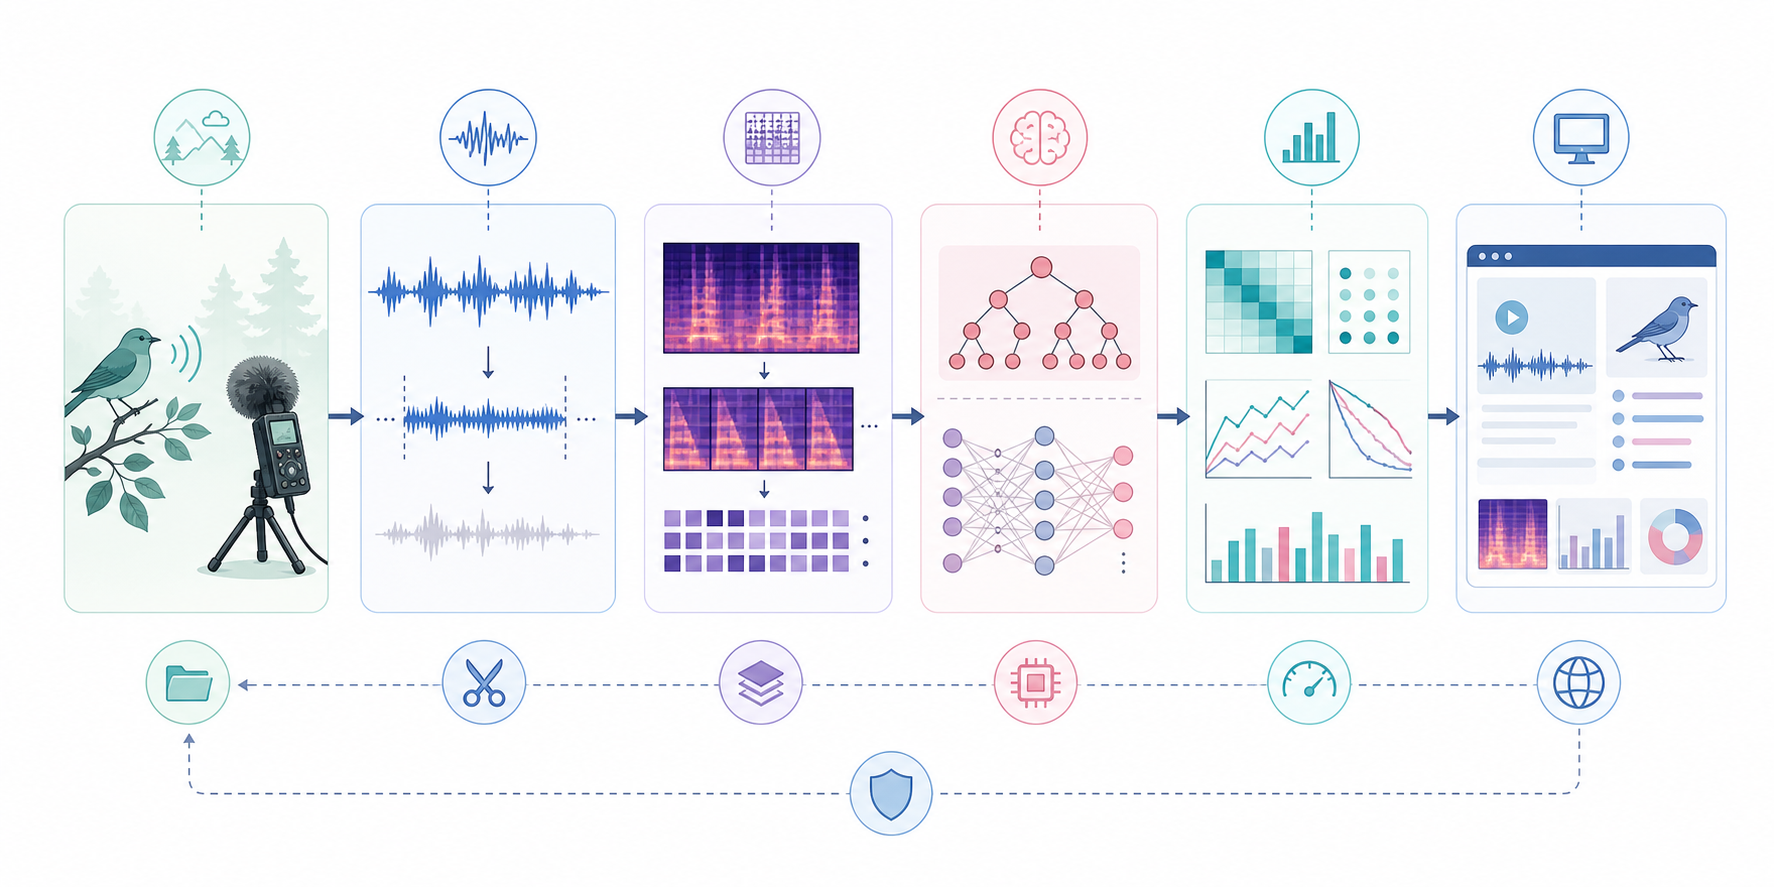
\includegraphics[width=0.96\textwidth]{figures/lsw_research_workflow.png}
\caption{鸟类声音识别实验流程示意。流程从野外声景采集开始，经过波形切片、频谱与 MFCC 特征提取、传统机器学习和神经网络建模，再到多标签指标评估与网页演示。图中只使用图标和箭头，具体含义由正文说明。}
\label{fig:research-workflow}
\end{figure}

\subsection{实验设计思路}
我们按课程要求组织实验，同时尽量让每个模块承担清楚的任务。评价指标没有只看单一准确率，而是采用 LRAP、label ranking loss、coverage error、hamming loss、micro/macro F1 和 Top-1 / Top-3 命中率，这样可以同时观察排序质量、阈值误差和用户看到的前几类预测结果。网页部分使用 FastAPI 提供接口，前端用原生 HTML、CSS 和 JavaScript 呈现实验看板和预测结果。模型方面，我们把传统机器学习作为主线，使用 ExtraTrees、Logistic Regression（L1）、KNN 和 Linear SVM；深度模型保留 CNN baseline 与 Attention-BiGRU，主要用于和频谱端到端路线做对照。

\subsection{研究目标}
我们的目标是完成一套可检查、可复现实验逻辑、可通过网页演示的鸟类声音识别系统。我们使用 BirdCLEF2026 数据集构建监督样本，提取 MFCC、pitch、volume、timbre、rate/onset 等声学特征，并分别训练传统机器学习模型和深度学习模型。模型评估采用 5 折交叉验证，结果以表格和图像形式保存。最后，我们把上传音频、Top-k 预测结果、波形、频谱和 MFCC 图放进网页界面中，方便课堂展示。

\section{数据集与任务建模}

\subsection{BirdCLEF2026 数据来源与监督对象}
BirdCLEF2026 提供训练录音、分类学元数据和声景标签。课程实验需要把音频输入和标签粒度对齐，因此我们没有直接使用整段长录音作为样本，而是使用与标签对应的 5 秒声景窗口。切分和去重后，最终得到 739 个唯一窗口，并在这些窗口上构建 75 个 active labels 的多标签监督矩阵。

如果直接把整段录音当作样本，标签粒度会和模型输入不一致；如果只保留单标签窗口，又会丢掉真实声景中的共现信息。因此，后续实验统一采用“5 秒短窗 + 多标签向量”的监督形式，传统模型和深度模型使用同一批样本。

\subsection{数据统计}
最终监督集的核心统计量见表~\ref{tab:dataset-stats}。窗口平均标签数为 4.2246，多标签窗口比例为 0.8945。也就是说，绝大多数 5 秒窗口都不只包含一种鸟声，单标签分类会简化问题本身。

\begin{table}[H]
\centering
\begin{tabular}{p{5.5cm}r}
\toprule
统计项 & 数值 \\
\midrule
唯一5秒窗口数 & 739.0000 \\
激活标签数 & 75.0000 \\
结构化特征维度 & 161.0000 \\
窗口平均标签数 & 4.2246 \\
窗口标签数中位数 & 4.0000 \\
多标签窗口比例 & 0.8945 \\
\bottomrule
\end{tabular}
\caption{监督数据集核心统计量}
\label{tab:dataset-stats}
\end{table}

\subsection{多标签建模的必要性}
若把本任务简化为单标签分类，会带来两个问题。第一，多个真实共现标签只能保留一个，标签信息被截断。第二，模型无法区分“第二高分标签也是正确标签”和“第二高分标签是误判”这两种情况。因此，我们将每个标签视为独立的 sigmoid 输出，并同时使用排序类指标和阈值类指标评估模型。

这一设计也决定了后续指标体系。比如 LRAP 衡量“正确标签是否被排在前面”，coverage error 衡量“要覆盖所有真实标签需要看多深”，而 hamming loss 则刻画每个标签位上的整体误报与漏报成本。相比传统的 Top-1 accuracy，这些指标更能反映多标签声景识别的真实性能。

形式化地说，给定第 $i$ 个 5 秒音频窗口 $x_i$，它对应的标签不是一个类别编号，而是一个 $C$ 维二值向量：
\begin{equation}
\mathbf{y}_i=(y_{i1},y_{i2},\ldots,y_{iC}),\quad y_{ic}\in\{0,1\},\quad C=75.
\end{equation}
模型输出每个类别的分数 $s_{ic}$，再通过 sigmoid 得到出现概率：
\begin{equation}
\hat{p}_{ic}=\sigma(s_{ic})=\frac{1}{1+\exp(-s_{ic})}.
\end{equation}
刚开始我们也考虑过只取最大概率类别，但这样会把一个声景窗口压成单标签问题。后来改成多标签向量以后，Top-k 预测和阈值预测都能自然解释，也更符合 BirdCLEF 声景数据本身。

\begin{figure}[H]
\centering
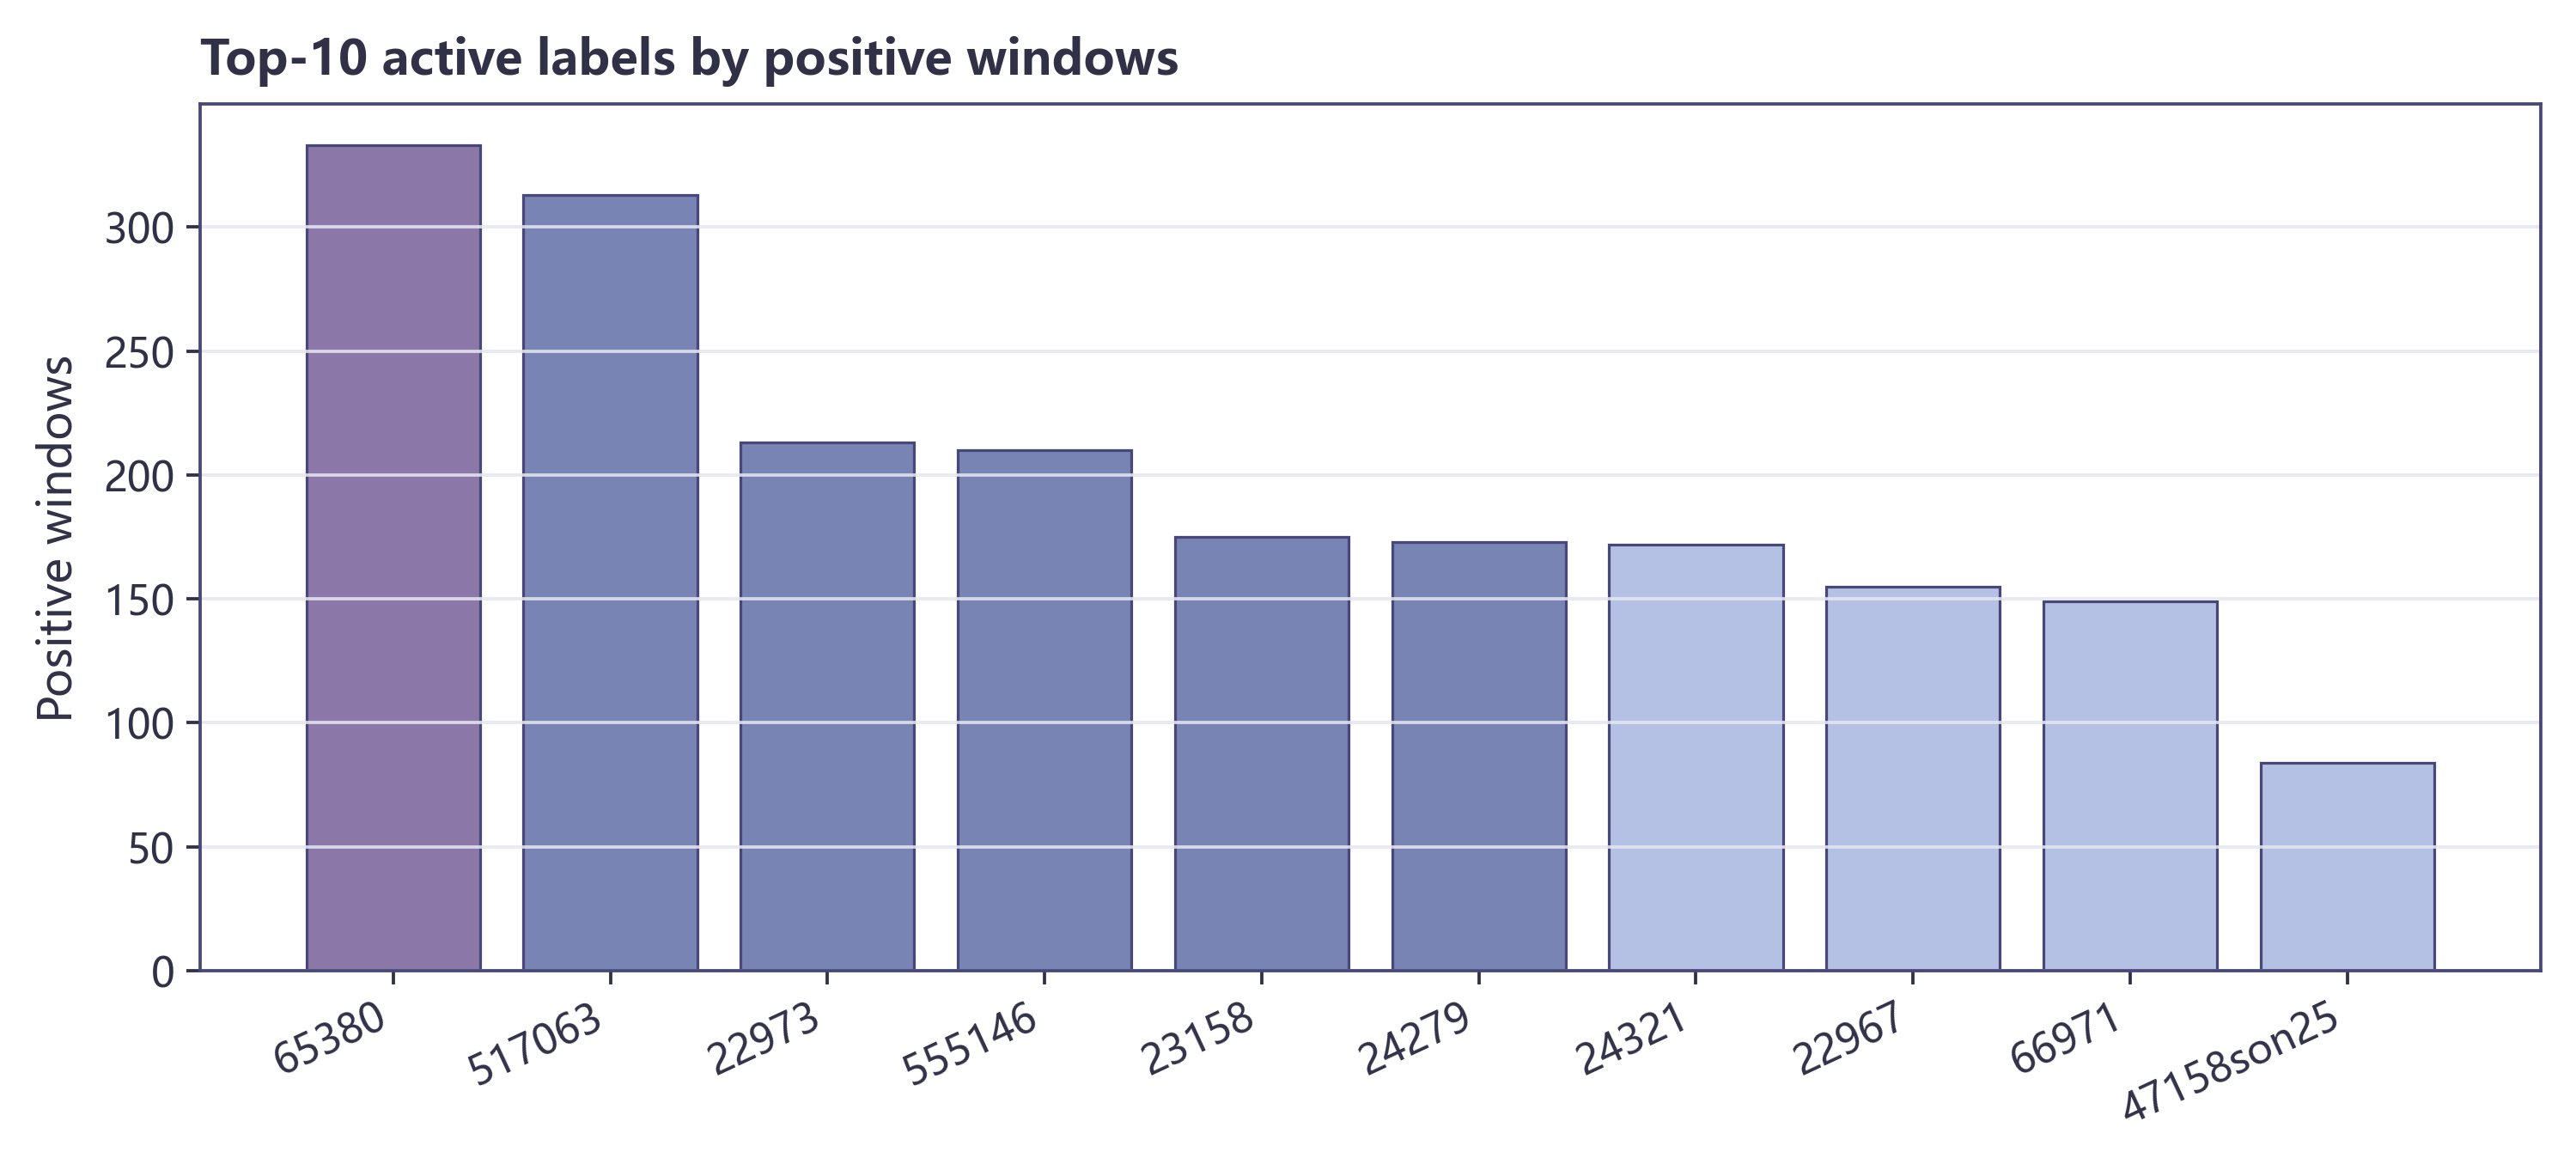
\includegraphics[width=0.86\textwidth]{figures/lsw_top_labels.png}
\caption{监督集中正样本窗口数最多的 Top-10 标签}
\label{fig:top-labels}
\end{figure}

\begin{figure}[H]
\centering
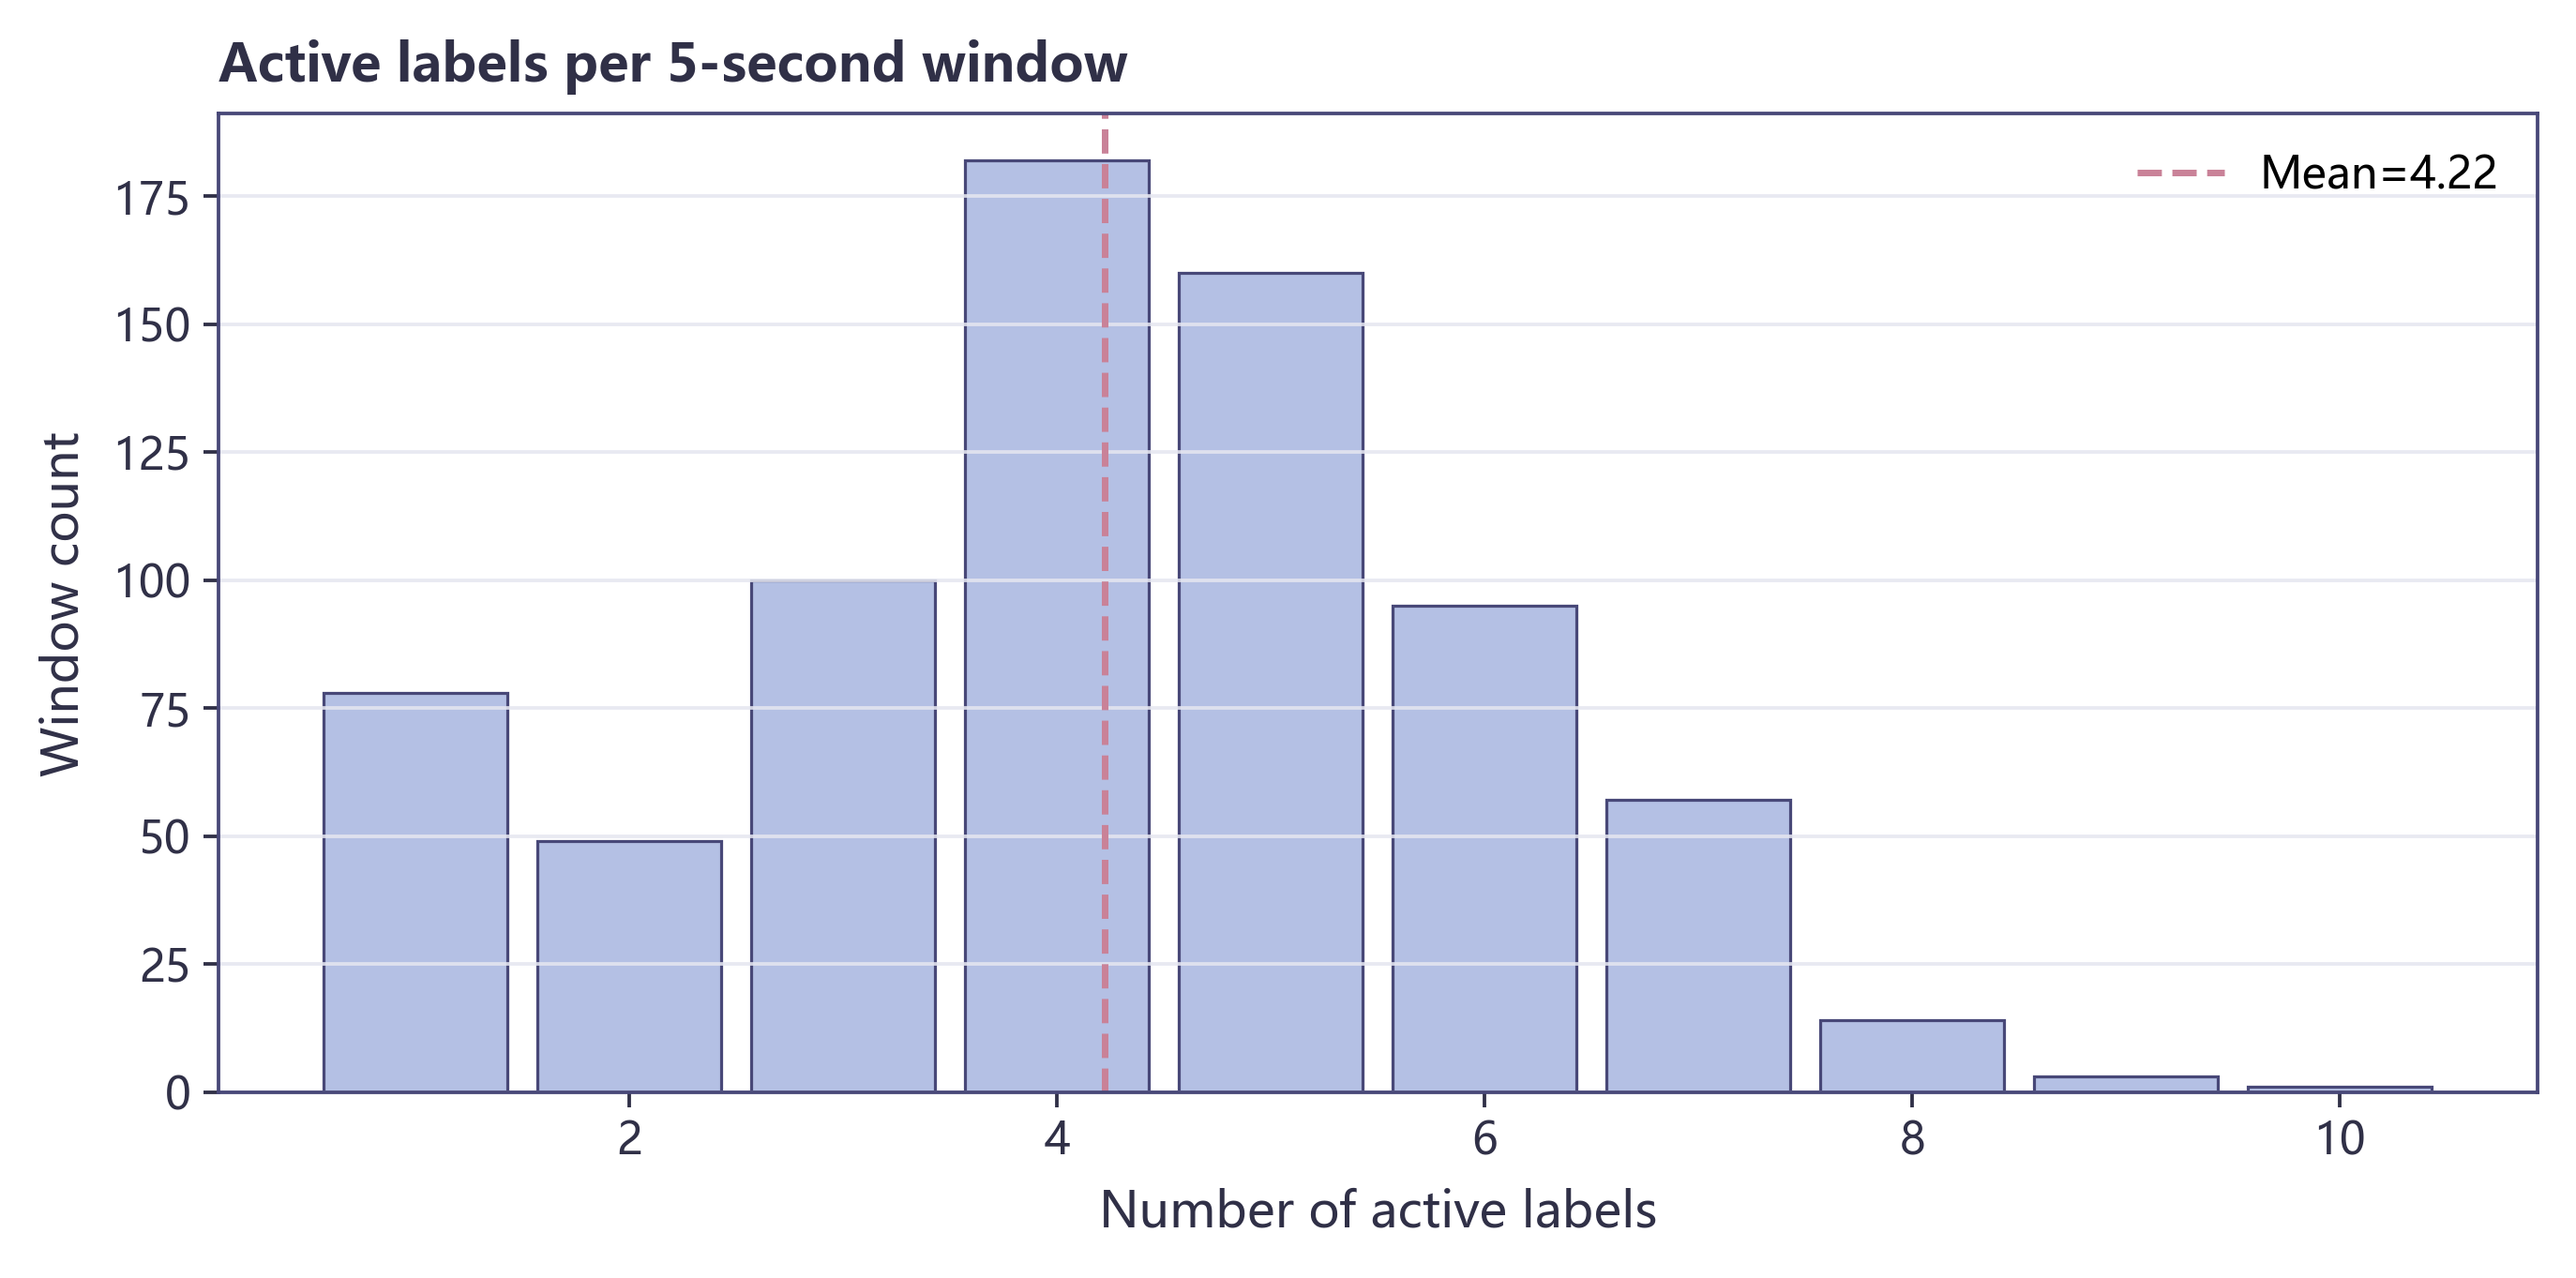
\includegraphics[width=0.82\textwidth]{figures/lsw_label_density.png}
\caption{每个 5 秒窗口包含的标签数量分布}
\label{fig:label-density}
\end{figure}

从图~\ref{fig:top-labels} 和图~\ref{fig:label-density} 可以看出，本任务同时具有类别分布不均衡和标签密度较高的特点。前者要求模型在训练中考虑 class imbalance，后者要求评价时使用适合多标签排序的指标。也正因为这两个特性并存，我们没有直接复用一般的多类单标签识别范式。

\subsection{样本窗口与标签构造说明}
我们把声景切成 5 秒窗口，是因为这个长度既能覆盖多数鸟鸣事件，又不会让背景噪声和无关片段占比过大。窗口太短时，一次完整鸣叫可能被截断，MFCC 和 pitch 等统计量会不稳定；窗口太长时，一个样本内会混入更多无关声音，模型更难判断哪些标签真正对应当前片段。5 秒窗口在 BirdCLEF 类任务中比较常见，也适合课堂实验中进行波形和频谱可视化。

标签构造时，我们没有把一个窗口强行压缩成一个类别，而是保留每个物种是否出现的二值向量。这样做会增加模型训练难度，但更符合真实声音识别场景。例如一个窗口里同时出现高频短促鸣叫和低频连续鸣叫，单标签建模只能留下其中一个类别；多标签建模则允许模型把两个候选都排在前面。后续网页展示 Top-k 结果时，这种设计也更合理，因为老师看到的是一组候选鸟类，而不是一个过度确定的单一答案。

\section{预处理与特征提取}

\subsection{预处理流程}
预处理分为四步。第一步，对原始音频统一做单声道化和 32kHz 重采样，避免采样率差异影响时频尺度。第二步，根据声景标签把长录音切成 5 秒窗口，过短样本补零，过长样本截断。第三步，依据窗口 ID 去重，减少重复样本对交叉验证的影响。第四步，基于窗口标签构建多标签矩阵，并筛出监督集中实际出现过的 75 个 active labels。

该流程同时服务于两条实验路线。传统机器学习分支使用定长结构化特征表；深度学习分支使用统一规格的 log-Mel 频谱缓存。统一的数据入口保证了模型对比更公平，避免“由于输入样本定义不同导致实验不可比”的问题。

\subsection{声学特征设计}
根据课程要求，我们显式保留了几类语音识别和音频识别中常用的声学信息。MFCC 及其一阶、二阶差分用于描述谱包络和短时动态变化，是很多传统语音识别系统都会使用的基础特征。Pitch 特征用 $f_0$ 的均值、标准差、最小值、最大值和 voiced ratio 近似描述周期性声源的主频变化。Volume 主要使用 RMS 统计和动态范围，反映声音强弱以及能量波动。Timbre 则通过谱质心、谱带宽、谱滚降、谱平坦度、谱对比度和过零率等统计量描述音色差异。Rate / Onset 用 onset 数量、onset rate、onset strength 与峰值计数近似表示鸣叫节奏和事件密度。

这些特征不是简单堆叠。我们选择它们，是因为它们分别对应了声音识别里常见的几个问题：声音的频谱包络是什么样，基音是否明显，能量是否集中，音色是否尖锐或宽厚，鸣叫节奏是否密集。与直接把频谱像素全部交给模型相比，结构化声学特征更容易解释，也更适合当前样本量偏小的课程实验。

\begin{table}[H]
\centering
\begin{tabular}{p{3.0cm}rp{7.8cm}}
\toprule
特征家族 & 维度 & 说明 \\
\midrule
基础统计 & 2 & duration\_sec, sample\_rate \\
MFCC及差分 & 120 & 20个MFCC + 一阶/二阶差分统计 \\
音高Pitch & 5 & f0\_mean/std/min/max + voiced\_ratio \\
音量Volume & 4 & rms\_mean/std/max + dynamic\_range \\
音色Timbre & 24 & 谱质心/带宽/滚降/平坦度/谱对比度/ZCR \\
节奏Rate & 6 & onset\_count/rate/strength + peak\_count/rate \\
\bottomrule
\end{tabular}
\caption{结构化特征家族与维度组成}
\label{tab:feature-families}
\end{table}

表~\ref{tab:feature-families} 显示，161 维特征中大部分来自 MFCC 及其差分统计，说明频谱包络信息在本实验中占主要位置。pitch、volume、timbre 和 onset/rate 则补充描述了音高、能量、音色和节奏变化。

\subsection{深度学习输入表示}
深度模型不直接使用上述 161 维结构化特征，而是使用二维 log-Mel 频谱。具体而言，系统将每个 5 秒窗口变换为 128 维 Mel 频带的时频矩阵，再做对数压缩。这样做有两个原因。第一，CNN 和时序模型更适合从局部时频纹理中学习模式；第二，log-Mel 表示天然保留了时间维度，有利于建模鸣叫片段的重复和变化。

\begin{figure}[H]
\centering
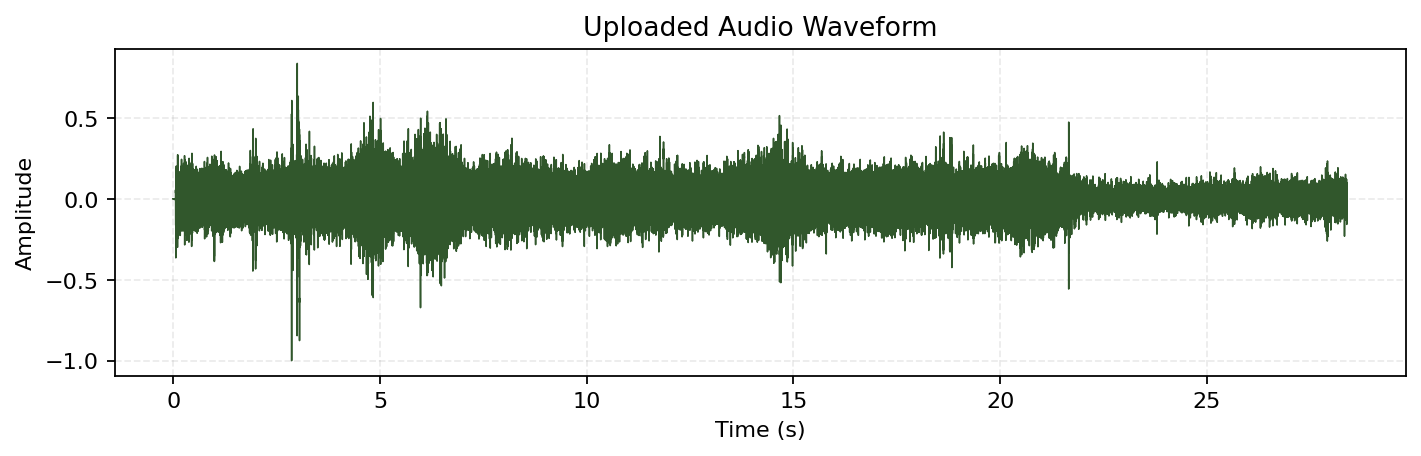
\includegraphics[width=0.31\textwidth]{figures/lsw_ui_waveform.png}\hfill
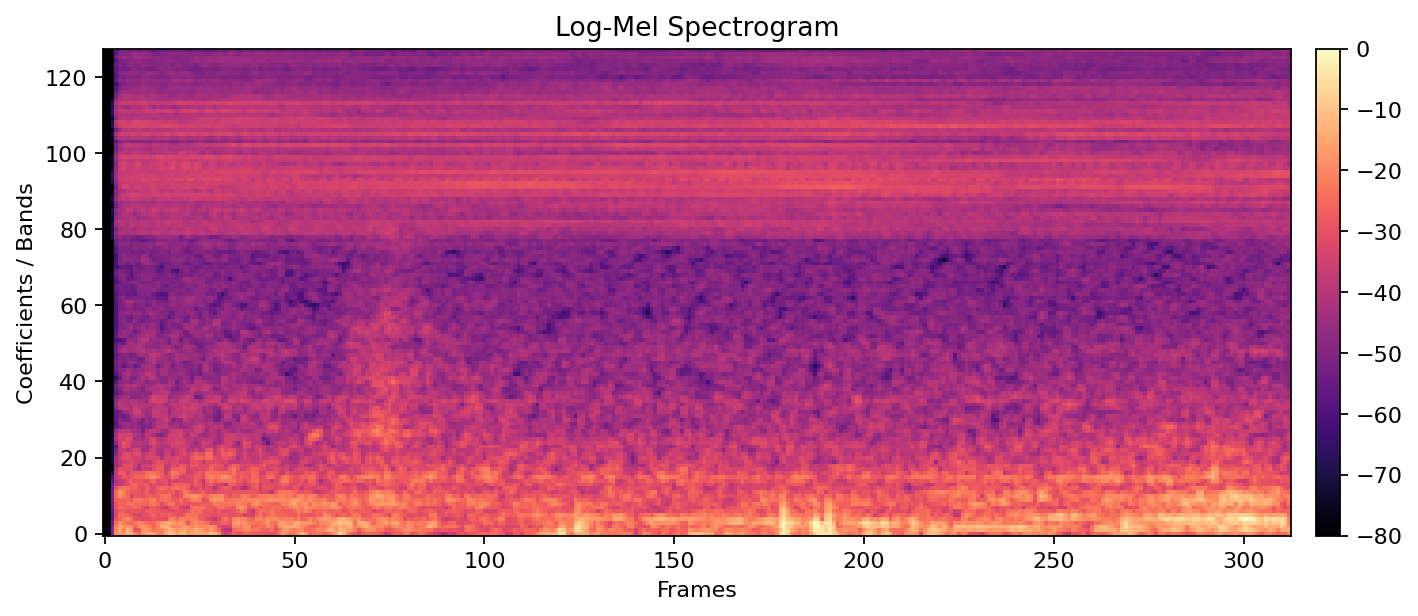
\includegraphics[width=0.31\textwidth]{figures/lsw_ui_logmel.png}\hfill
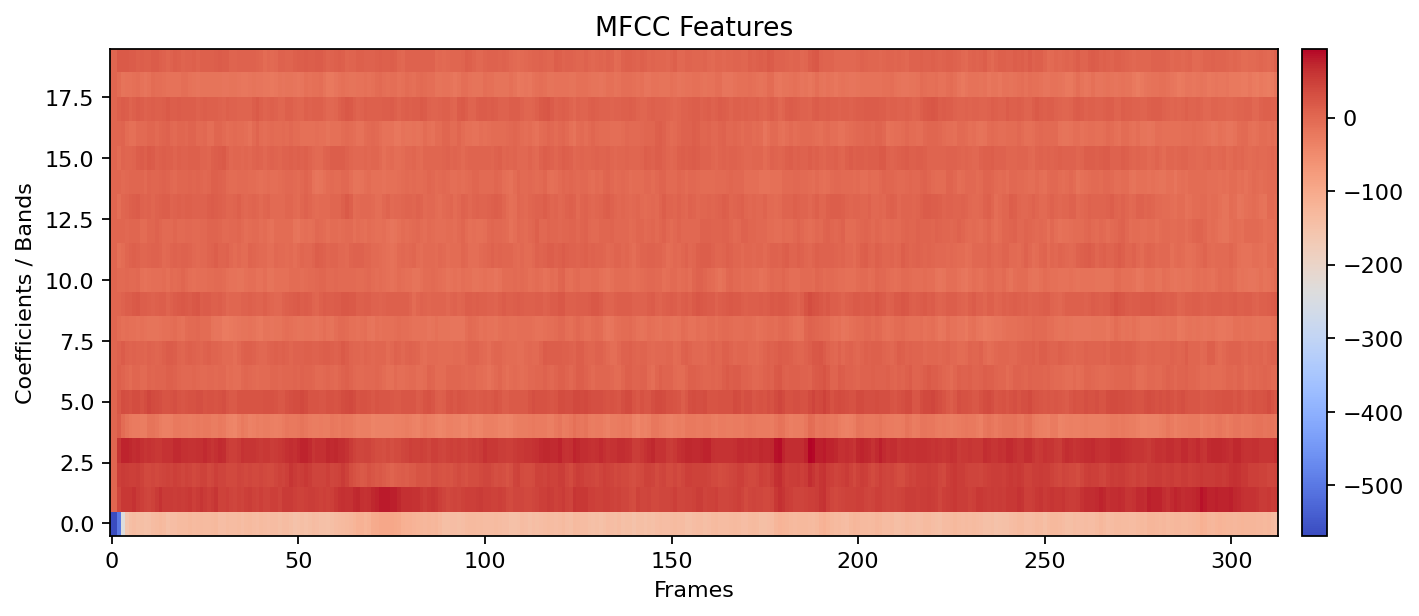
\includegraphics[width=0.31\textwidth]{figures/lsw_ui_mfcc.png}
\caption{网页演示样例的波形、Log-Mel 频谱和 MFCC 特征图}
\label{fig:ui-audio-views}
\end{figure}

图~\ref{fig:ui-audio-views} 给出了网页系统在一次示例预测中返回的三类图像：波形图、Log-Mel 频谱图和 MFCC 图。波形可以观察音量变化，Log-Mel 频谱保留时间和频率结构，MFCC 图则对应传统特征中的谱包络信息。

\subsection{特征与声音现象的对应关系}
MFCC 的作用可以理解为把频谱形状压缩成一组较低维的系数。语音识别中，MFCC 常用来描述声道滤波后的谱包络；在鸟鸣识别里，它也能描述不同鸣叫的频率分布轮廓。我们同时加入一阶差分和二阶差分，是为了补充短时变化速度和变化趋势。某些鸟鸣不是稳定长音，而是快速上滑、下滑或颤动，只看静态 MFCC 会丢掉这类动态信息。

Pitch 特征主要对应声音的基频。并不是所有鸟鸣都有清晰基频，噪声型或很短促的鸣叫可能会让 pitch 估计不稳定，所以我们没有把 pitch 当作唯一依据，而是只把它作为一组补充统计量。Volume 特征反映声音能量变化，可以帮助区分连续稳定鸣叫和短促爆发声。Timbre 特征更接近音色描述，谱质心偏高通常意味着声音更尖锐，谱带宽和谱对比度可以反映频谱分布是否集中。Onset 和 rate 则描述鸣叫事件的出现节奏，它们对重复型鸣叫尤其有帮助。

从课程要求看，这些特征覆盖了“梅尔频率倒谱系数、音高、音量、音色和语速/速率”等核心知识点。我们在网页中同时展示波形、Log-Mel 和 MFCC，也是为了让这些概念能被直观看到：波形看能量，频谱看时间和频率，MFCC 看压缩后的谱包络。报告中的模型指标只是最终结果，真正体现声音识别知识点的是从音频到特征的这一段处理过程。

在实现上，音频窗口会先经过短时傅里叶变换：
\begin{equation}
X(m,k)=\sum_{n=0}^{N-1}x[n+mH]w[n]\exp\left(-j\frac{2\pi kn}{N}\right),
\end{equation}
其中 $w[n]$ 是窗函数，$H$ 是 hop length。Mel 频谱可以看作把线性频率上的能量投影到更符合听觉感知的 Mel 滤波器组：
\begin{equation}
E_b=\sum_k |X(m,k)|^2 M_b(k).
\end{equation}
MFCC 则是在对数 Mel 能量上做离散余弦变换：
\begin{equation}
c_q=\sum_{b=1}^{B}\log(E_b)\cos\left[\frac{\pi q}{B}\left(b-\frac{1}{2}\right)\right].
\end{equation}
这几步让我们把原始波形、频谱能量和倒谱系数连起来，也解释了为什么 MFCC 会比直接使用波形更适合传统机器学习模型。图 \ref{fig:research-workflow} 中的波形、频谱块和特征矩阵，对应的就是这一段从连续声音到结构化特征的转换过程。

\section{模型构建与实验设置}

\subsection{传统机器学习模型}
传统机器学习部分使用 ExtraTrees、Logistic Regression（L1）、KNN 和 Linear SVM 四个模型。ExtraTrees 使用 260 棵树，并设置 balanced 类别权重，用来处理多标签任务中的类别不平衡。Logistic Regression（L1）配合标准化和 One-vs-Rest，可以观察稀疏线性判别在这组声学特征上的效果。KNN 采用距离加权，作为局部邻域方法的对照；Linear SVM 则提供线性最大间隔模型的结果。

这四类模型的假设不同。ExtraTrees 更适合处理非线性特征组合，Logistic Regression 和 Linear SVM 属于线性判别模型，KNN 则依赖特征空间中的局部距离。我们把它们放在同一套声学特征上比较，是为了判断这些 MFCC、音高、音量、音色和节奏特征到底更适合哪类分类器。

\subsection{深度学习模型}
深度学习部分保留两个模型，主要作为频谱端到端路线的对照。CNN baseline 对 log-Mel 频谱做二维卷积，关注局部时频纹理；Attention-BiGRU 先用 CNN 压缩频带维度，再用双向 GRU 建模时间序列，并通过 attention 汇聚重要时间片的信息。我们没有把深度模型作为报告主结论，因为当前监督窗口只有 739 个，直接训练频谱模型容易受到样本规模限制。保留这一部分，是为了说明同一批音频数据在“手工声学特征”和“频谱端到端学习”两条路线上的差别。

\subsection{训练与优化设置}
所有模型统一采用 5 折交叉验证。传统模型通过 OOF 分数进行全局阈值搜索；深度模型使用 BCEWithLogitsLoss，并根据训练折标签分布构造 \texttt{pos\_weight}，以减轻类别不平衡的影响。远程 GPU 训练使用 4090D 显卡，深度学习最大训练轮数设为 10，batch size 为 256，dropout 为 0.35，优化器使用 AdamW，并通过 ReduceLROnPlateau 调整学习率。为了避免无效训练，深度模型还使用早停策略；Attention-BiGRU 分支额外加入了简单 SpecAugment，用来模拟频谱遮挡。

网页推理与远程训练分开使用计算资源。训练阶段优先使用 GPU；网页服务中的推理默认走 CPU，避免影响深度模型训练。这个设置不改变实验结论，但能保证训练和网页演示同时保留。

深度模型的目标函数使用多标签 BCE 形式。对一个 batch 来说，可以写成：
\begin{equation}
\mathcal{L}_{BCE}=-\frac{1}{BC}\sum_{i=1}^{B}\sum_{c=1}^{C}
\left[y_{ic}\log\hat{p}_{ic}+(1-y_{ic})\log(1-\hat{p}_{ic})\right].
\end{equation}
后来训练时我们发现，直接训练会让模型偏向常见类别，所以加入 \texttt{pos\_weight}。这个调整不能保证深度模型一定变好，但它至少把“少数类正样本太少”的问题纳入了优化过程。

\subsection{模型对比的公平性}
为了让模型对比有意义，我们尽量保证不同模型使用同一批监督窗口和同一套交叉验证划分。传统模型和深度模型的输入形式不同，一个使用 161 维结构化声学特征，另一个使用 log-Mel 频谱，但标签矩阵、折划分和主评价指标保持一致。这样得到的差异更接近“特征路线和模型路线的差异”，而不是数据划分或评价方式造成的差异。

传统模型的训练速度明显快于深度模型，但我们没有因此只保留传统模型。课程要求同时包含传统机器学习和深度学习算法，所以两条路线都要完成。深度模型结果较弱时，我们也没有删除它，而是保留训练曲线、fold 结果和阈值优化结果。这样做可以说明实验过程是真实的，也能让报告更完整地解释为什么最终主结果选择传统声学特征路线。

\subsection{评价指标体系}
我们使用多标签排序指标和阈值指标共同评价模型，而不只看单一 AUC。LRAP 反映真实标签在预测排序中是否靠前，label ranking loss 则衡量错误排序比例。coverage error 表示平均需要查看多少个预测标签才能覆盖全部真实标签，hamming loss 反映每个标签位上的误报和漏报。micro/macro F1 分别从总体标签层面和类别均衡层面评估模型，Top-1 / Top-3 hit rate 则更接近网页演示时用户的直观体验：前几个候选类别里有没有命中真实鸟类。

这套指标比单纯准确率更适合当前任务。多标签声景中，一个窗口可能有多个正确标签，因此需要同时看排序质量、阈值误差和 Top-k 命中情况。

这些指标的侧重点并不相同。LRAP 高，说明模型通常能把真实鸟类排在较靠前的位置，适合评价“候选列表是否有用”。Hamming Loss 低，说明在 75 个标签位上，模型整体误报和漏报较少。Micro F1 更受高频类别影响，能反映总体预测能力；Macro F1 会让低频类别也有同等权重，因此在类别不均衡时通常更难提升。Top-3 命中率适合网页演示，因为用户实际查看结果时往往会先看前几个候选，而不是逐个检查 75 个标签。

我们没有把 macro ROC-AUC 或 mAP 作为主指标，是为了和已有版本做出区分，也为了让报告更贴近多标签排序和课堂展示场景。比如老师上传一段鸟鸣后，最关心的是系统给出的前几类是否合理、是否能看到声音特征图，而不是单独询问每个标签的 ROC 曲线。因此，LRAP、Top-k 命中率和 Hamming Loss 更适合作为这次网页系统的主说明指标。

其中 Hamming Loss 和 Top-k hit rate 的计算很直观：
\begin{equation}
\mathrm{HL}=\frac{1}{NC}\sum_{i=1}^{N}\sum_{c=1}^{C}\mathbb{I}(\hat{y}_{ic}\ne y_{ic}),
\end{equation}
\begin{equation}
\mathrm{Top}\mbox{-}k=\frac{1}{N}\sum_{i=1}^{N}\mathbb{I}\left(\mathrm{TopK}(\hat{\mathbf{p}}_i)\cap \{c:y_{ic}=1\}\ne\varnothing\right).
\end{equation}
Micro F1 则把所有标签位放在一起统计：
\begin{equation}
\mathrm{Micro\ F1}=\frac{2TP}{2TP+FP+FN}.
\end{equation}
我们在第一次整理结果时发现，只看 Top-1 会让部分多标签窗口显得“不准”，但 Top-3 能体现候选列表是否覆盖真实鸟类。因此最后报告同时保留阈值类指标和排序类指标，而不是只选一个最好看的分数。图 \ref{fig:research-workflow} 右侧的指标面板和网页窗口，也对应了我们最终展示时希望老师看到的内容：不仅有预测类别，还有识别过程中的声学证据和模型对比。

\section{实验结果}

\subsection{总体结果}
最终总表见表~\ref{tab:model-summary}。四个传统模型的结果都高于两个深度模型，其中 ExtraTrees 的 LRAP 为 0.9329，Micro F1 为 0.8862，Top-3 命中率为 0.9878，是本次实验的综合最优模型。深度模型中，CNN baseline 略优于 Attention-BiGRU，但两者都没有达到传统模型的水平。

\begin{table}[H]
\centering
\resizebox{\textwidth}{!}{\begin{tabular}{lrrrrrr}
\toprule
Model & LRAP & Micro F1 & Macro F1 & Top-3 & Hamming & Thr \\
\midrule
extra\_trees & 0.9329 & 0.8861 & 0.5755 & 0.9878 & 0.0123 & 0.4500 \\
logistic\_regression\_l1 & 0.9011 & 0.8251 & 0.5737 & 0.9865 & 0.0213 & 0.8000 \\
knn\_distance & 0.8954 & 0.8448 & 0.5210 & 0.9702 & 0.0167 & 0.4500 \\
linear\_svm & 0.8561 & 0.7330 & 0.5394 & 0.9770 & 0.0350 & 0.5500 \\
cnn\_baseline\_lsw & 0.0871 & 0.0835 & 0.0497 & 0.1487 & 0.5722 & 0.4000 \\
attention\_bigru & 0.0718 & 0.0747 & 0.0478 & 0.0487 & 0.6123 & 0.3500 \\
\bottomrule
\end{tabular}}
\caption{六个模型的最终指标总表}
\label{tab:model-summary}
\end{table}

\begin{figure}[H]
\centering
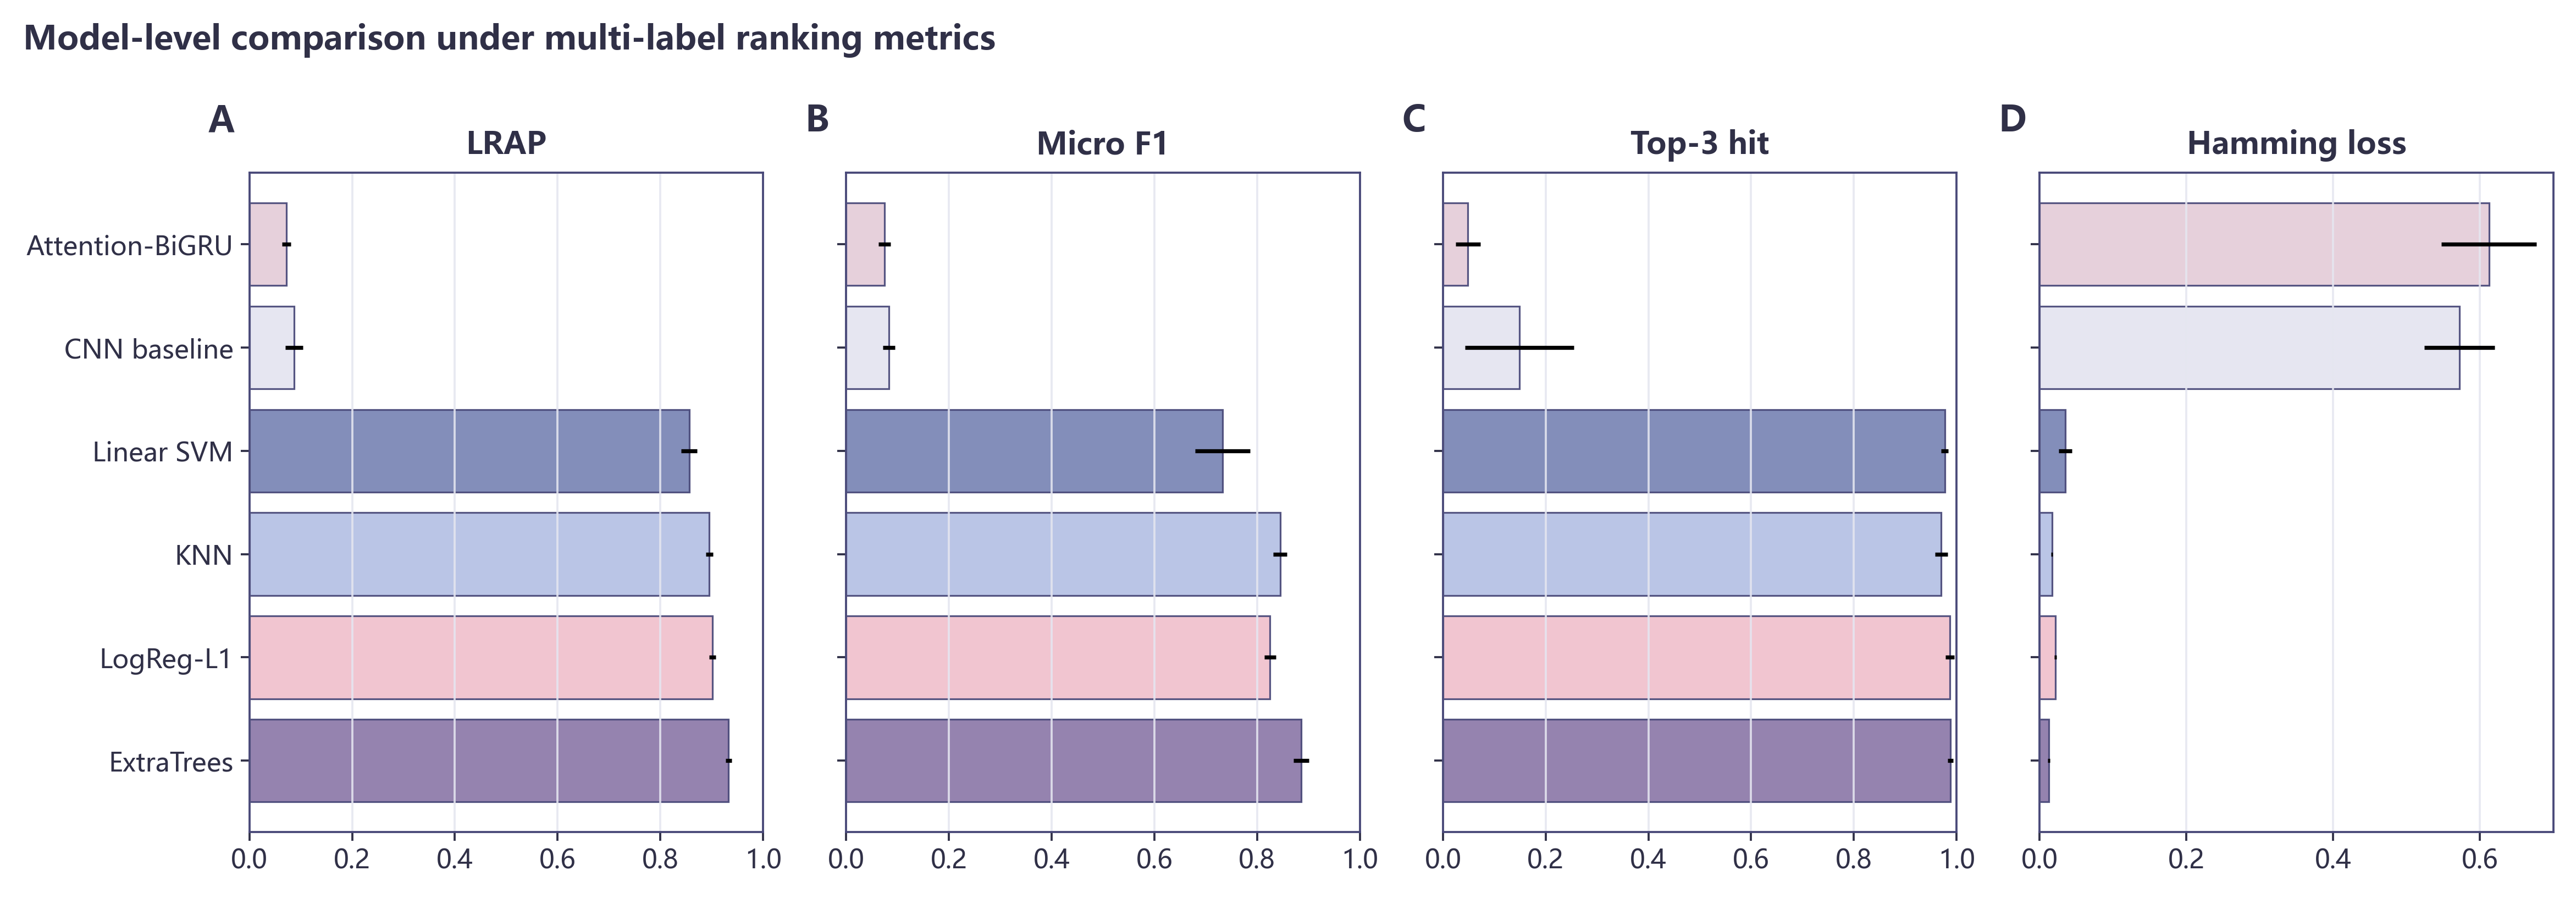
\includegraphics[width=\textwidth]{figures/lsw_model_overview.png}
\caption{六个模型在 LRAP、Micro F1、Top-3 命中率和 Hamming Loss 上的对比}
\label{fig:model-overview}
\end{figure}

\begin{figure}[H]
\centering
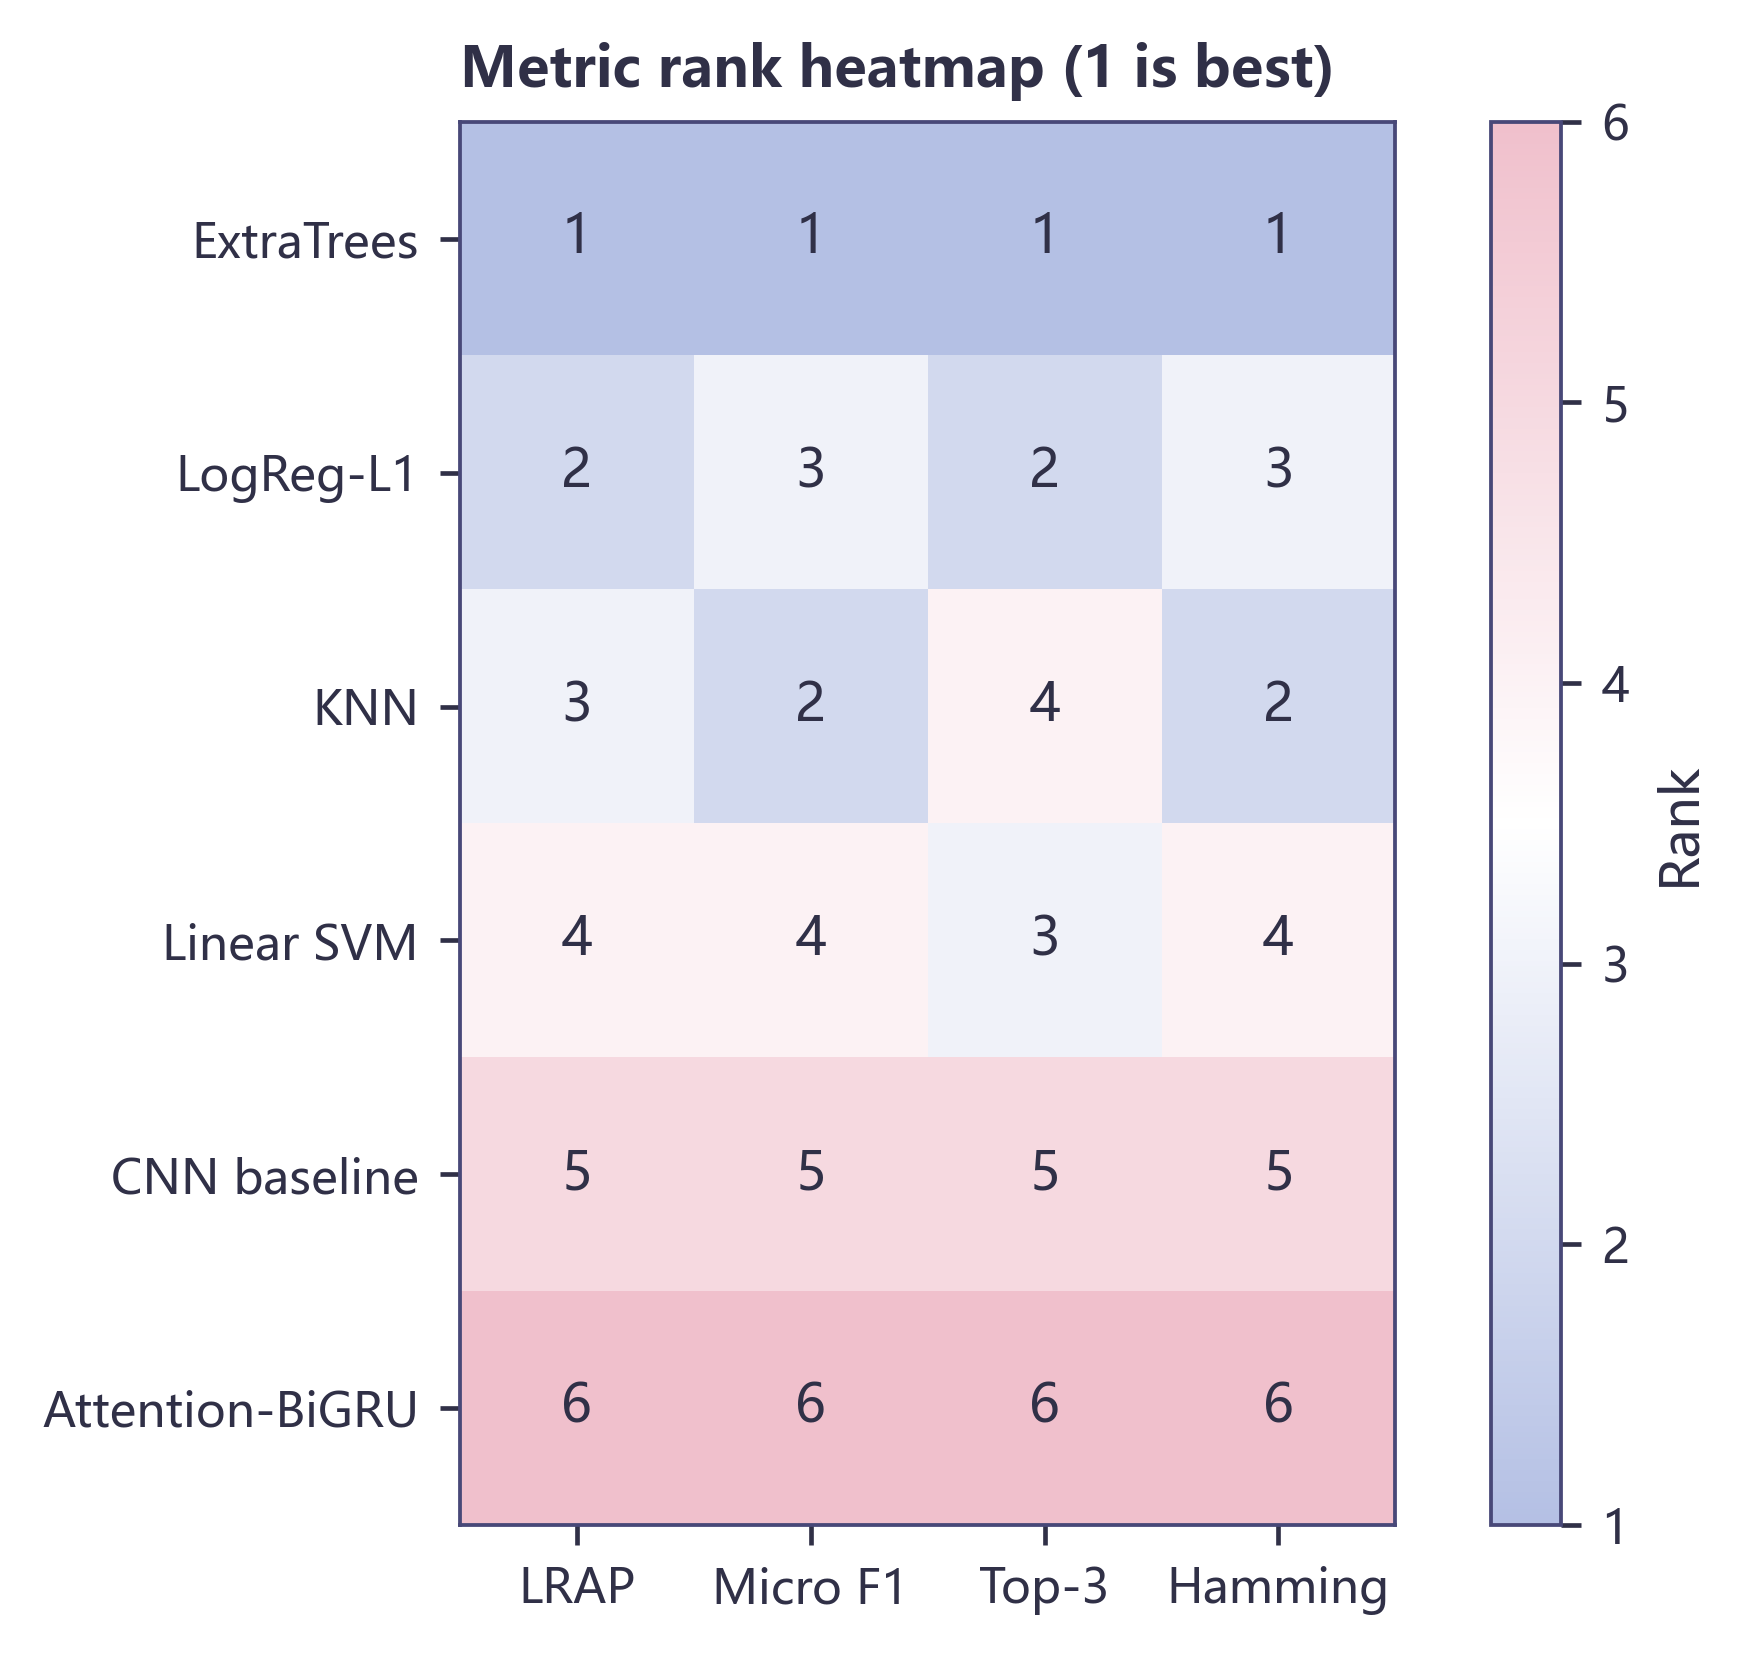
\includegraphics[width=0.82\textwidth]{figures/lsw_metric_rank_heatmap.png}
\caption{六个模型在四个核心指标上的排名热图，数值 1 表示该指标下排名最好}
\label{fig:metric-rank-heatmap}
\end{figure}

图~\ref{fig:model-overview} 和图~\ref{fig:metric-rank-heatmap} 反映出两个现象。传统模型整体得分较高，说明 161 维结构化特征已经包含了较多可用信息。深度模型的 Hamming Loss 较高，说明它们在全标签维度上存在较多误报和漏报，这与当前样本量偏小有关。排名热图也让这个结论更直观：ExtraTrees 不只是某一个指标高，而是在多个关键指标上都比较靠前。

如果从声音识别角度解释这个结果，传统模型表现更好并不是因为它“更复杂”，而是因为输入特征已经把很多声学知识提前编码进去了。MFCC 把频谱包络压缩成稳定统计量，pitch 和 volume 提供主频与能量信息，timbre 和 onset/rate 补充音色和节奏。ExtraTrees 这类树模型能够在这些统计量之间学习非线性组合，所以在小样本情况下更容易取得稳定分数。深度模型虽然理论上可以从 log-Mel 频谱中自动学习特征，但它需要更多样本覆盖不同噪声、录音设备和物种变化，否则容易学不到稳定模式。

我们在解释结果时更看重“哪条技术路线适合当前数据”。从表~\ref{tab:model-summary} 看，传统模型不仅 LRAP 高，Top-3 命中率也接近 0.99。这说明在多数窗口中，真实标签至少能出现在靠前候选里。网页演示时，这一点很重要，因为系统输出的是 Top-k 识别结果，Top-k 候选质量比单个最大概率类别更能反映系统可用性。

\subsection{传统机器学习结果分析}
传统机器学习中，ExtraTrees 的结果最好。它在 LRAP、Micro F1、Top-1 和 Top-3 指标上均领先，阈值优化后的预测密度约为 0.0545，与真实多标签密度比较接近。Linear SVM 的 Top-3 命中率也较高，但 Hamming Loss 更大，说明线性边界对这组声学统计特征的利用不如树模型充分。

\begin{figure}[H]
\centering

\includegraphics[width=\textwidth]{figures/lsw_classical_model_comparison.png}
\caption{传统机器学习模型对比图}
\label{fig:classical-models}
\end{figure}

图~\ref{fig:classical-models} 说明，模型复杂度不是唯一因素。树模型可以处理结构化声学统计量中的非线性关系，因此在这组特征上比线性模型更占优势。

Logistic Regression 和 Linear SVM 的表现也有参考价值。它们的分数低于 ExtraTrees，但并没有完全失效，说明这些声学特征本身已经具备一定线性可分性。KNN 的结果介于两者之间，它依赖特征空间距离，如果同类鸟鸣在 MFCC、音色和节奏统计上聚得比较近，就能取得较好效果；但当背景噪声或多标签共现导致样本混杂时，邻域方法容易受到干扰。综合来看，ExtraTrees 更适合当前“特征维度较高、样本数不大、类别关系非线性”的数据形态。

\subsection{阈值优化结果}
阈值优化结果见表~\ref{tab:thresholds}。传统模型的最优阈值大多位于 0.45--0.80，而两个深度模型的最优阈值分别降到 0.40 和 0.35。这并不表示深度模型更好，而是说明它们的概率输出校准较差，必须通过较低阈值才能勉强拉起一部分正例召回。

\begin{table}[H]
\centering
\resizebox{0.82\textwidth}{!}{\begin{tabular}{lrrrr}
\toprule
Model & Threshold & LRAP & Micro F1 & Pred density \\
\midrule
extra\_trees & 0.4500 & 0.9329 & 0.8917 & 0.0545 \\
logistic\_regression\_l1 & 0.8000 & 0.9011 & 0.8438 & 0.0530 \\
knn\_distance & 0.4500 & 0.8954 & 0.8500 & 0.0527 \\
linear\_svm & 0.5500 & 0.8561 & 0.8203 & 0.0548 \\
cnn\_baseline\_lsw & 0.4000 & 0.0871 & 0.1075 & 0.9883 \\
attention\_bigru & 0.3500 & 0.0719 & 0.1067 & 0.9990 \\
\bottomrule
\end{tabular}}
\caption{最终阈值优化结果}
\label{tab:thresholds}
\end{table}

\begin{figure}[H]
\centering

\includegraphics[width=0.76\textwidth]{figures/lsw_threshold_optimization.png}
\caption{传统模型最优阈值对比}
\label{fig:thresholds}
\end{figure}

深度模型在阈值优化后的预测密度接近 1。如果只依赖全局阈值修正其输出，模型容易把大量标签判为正例。这说明问题主要出在排序和校准能力上，而不是单纯的阈值取值问题。

阈值优化在多标签识别里很关键。模型输出的是每个标签的概率或分数，但最终是否判为出现，需要一个阈值。如果阈值太高，模型会漏掉弱鸟声；如果阈值太低，又会把背景声或相似鸟声误判成正例。我们采用全局阈值搜索，是一种简单但清楚的优化方式，能让不同模型在同一评价标准下比较。后续如果继续改进，可以对每个物种单独设置阈值，因为高频常见鸟和低频少见鸟的最佳阈值通常不同。

\subsection{深度学习结果分析}
深度模型汇总结果表明，CNN baseline 的 LRAP 为 0.0871，Attention-BiGRU 的 LRAP 为 0.0718；二者的 Micro F1 分别只有 0.0835 和 0.0747，远低于传统模型。Attention-BiGRU 引入了时序建模和注意力汇聚，但在当前样本量下没有带来明显提升。

\begin{table}[H]
\centering
\resizebox{0.90\textwidth}{!}{\begin{tabular}{lrrrrr}
\toprule
Model & Fold & Best epoch & LRAP & Micro F1 & Top-3 \\
\midrule
attention\_bigru & 1 & 3 & 0.0792 & 0.0970 & 0.0473 \\
attention\_bigru & 2 & 1 & 0.0649 & 0.0714 & 0.0068 \\
attention\_bigru & 3 & 4 & 0.0692 & 0.0653 & 0.0541 \\
attention\_bigru & 4 & 4 & 0.0843 & 0.0648 & 0.0811 \\
attention\_bigru & 5 & 2 & 0.0615 & 0.0750 & 0.0544 \\
cnn\_baseline\_lsw & 1 & 1 & 0.0869 & 0.1018 & 0.1284 \\
cnn\_baseline\_lsw & 2 & 1 & 0.1173 & 0.0891 & 0.3108 \\
cnn\_baseline\_lsw & 3 & 4 & 0.0871 & 0.0662 & 0.2230 \\
cnn\_baseline\_lsw & 4 & 4 & 0.0766 & 0.0832 & 0.0203 \\
cnn\_baseline\_lsw & 5 & 3 & 0.0673 & 0.0770 & 0.0612 \\
\bottomrule
\end{tabular}}
\caption{深度学习各折结果与最优 epoch}
\label{tab:deep-folds}
\end{table}

\begin{figure}[H]
\centering

\includegraphics[width=0.82\textwidth]{figures/lsw_deep_model_comparison.png}
\caption{深度学习模型汇总对比}
\label{fig:deep-summary}
\end{figure}

\begin{figure}[H]
\centering

\includegraphics[width=0.84\textwidth]{figures/lsw_deep_training_curves.png}
\caption{深度学习验证损失曲线}
\label{fig:deep-curves}
\end{figure}

结合表~\ref{tab:deep-folds} 和图~\ref{fig:deep-curves}，多个折次在第 1--4 个 epoch 就达到最优验证性能，之后继续训练并没有带来稳定提升。这说明当前限制主要来自样本规模和标签结构，而不是 GPU 算力不足。

从训练曲线看，验证损失在后半段出现波动，说明模型并没有稳定学到可以泛化的频谱模式。Attention-BiGRU 增加了时序建模能力，但参数和结构也更复杂，在样本不足时不一定比简单 CNN 更好。这个现象和很多语音识别/音频识别任务是一致的：深度网络不是只要有 GPU 就一定更优，它需要足够数据、合适的数据增强和更可靠的标签质量。当前实验中，深度模型的意义主要是完成课程要求中的深度学习建模，并作为频谱端到端路线的对照。

\subsection{为什么深度模型显著弱于传统模型}
从实验结果看，深度模型落后并不意外。我们最终使用的监督窗口只有 739 个，却要预测 75 个标签，平均到每个类别上的正样本数量并不充足。另一方面，每个窗口平均有 4 个以上标签，近九成窗口都是多标签样本，这会增加端到端模型的优化难度。相比之下，传统模型使用的 161 维结构化特征已经把频谱、基音、能量、音色和节奏信息压缩成了比较稳定的统计量，小样本条件下更容易被树模型利用。

深度模型还有一个明显问题：阈值优化后预测密度接近 1，说明模型倾向于把大量标签判成正例。降低阈值可以提高一部分召回，但无法真正解决排序和概率校准问题。因此，我们没有把深度学习简单判定为无效，而是把它解释为频谱端到端路线的对照结果。对本次课程实验来说，结构化声学特征加传统模型更稳，也更容易向老师解释。

\subsection{误差来源分析}
这次实验的误差主要来自三个方面。首先是标签噪声和声景混叠。BirdCLEF 声景数据来自真实环境，同一个窗口可能存在多只鸟、环境声和远距离弱声音，标签本身不一定能精确对应到最清晰的声源。即使模型预测出了一个听起来合理的相似鸟种，如果标签文件中没有记录，也会在评价中被当作错误。

其次是类别不均衡。Top-10 标签占据了较多正样本，而长尾类别的窗口数较少。传统模型能通过 class weight 和树模型分裂缓解一部分问题，但低频类别仍然很难学到稳定边界。Macro F1 明显低于 Micro F1，也反映了这一点：模型对总体常见标签识别较好，但对少数标签还不够稳定。

第三是声学特征和真实物种差异之间仍有距离。MFCC、pitch、volume、timbre 和 onset/rate 可以描述声音形态，但它们不是鸟类生物学意义上的完整鸣叫模式。两个物种如果叫声频率相近、节奏相似，模型仅凭短时统计量仍可能混淆。后续如果要进一步提高效果，可以加入更细粒度的时序统计、物种先验信息，或者使用预训练音频模型提取更稳健的嵌入表示。

\section{网页系统与可视化实现}

\subsection{系统结构}
网页系统由 FastAPI 提供后端接口，前端采用原生 HTML、CSS 和 JavaScript。我们设置了三个主要接口：\texttt{/api/dashboard} 返回实验总表、老师要求核对项和图表元数据；\texttt{/api/predict} 接收用户上传音频，执行模型推理并返回 Top-k 结果与特征图；\texttt{/api/predict-sample} 用来对预置样例音频直接推理，方便课堂演示与截图。

网页中的实验看板显示实验主题、数据集、实验状态、最优传统模型、指标总表、阈值优化表和老师要求核对表。这样页面既能完成上传识别，也能直接呈现实验主要结果。

\subsection{页面展示效果}
原来的整页截图内容太长，放在报告里不容易看清楚。我们改为按模块截图：顶部概览和音频上传区单独展示，模型指标看板单独展示，老师要求核对表单独展示，实验图表也单独截取。这样老师查看报告时可以直接看到每个模块对应的功能。

\begin{figure}[H]
\centering
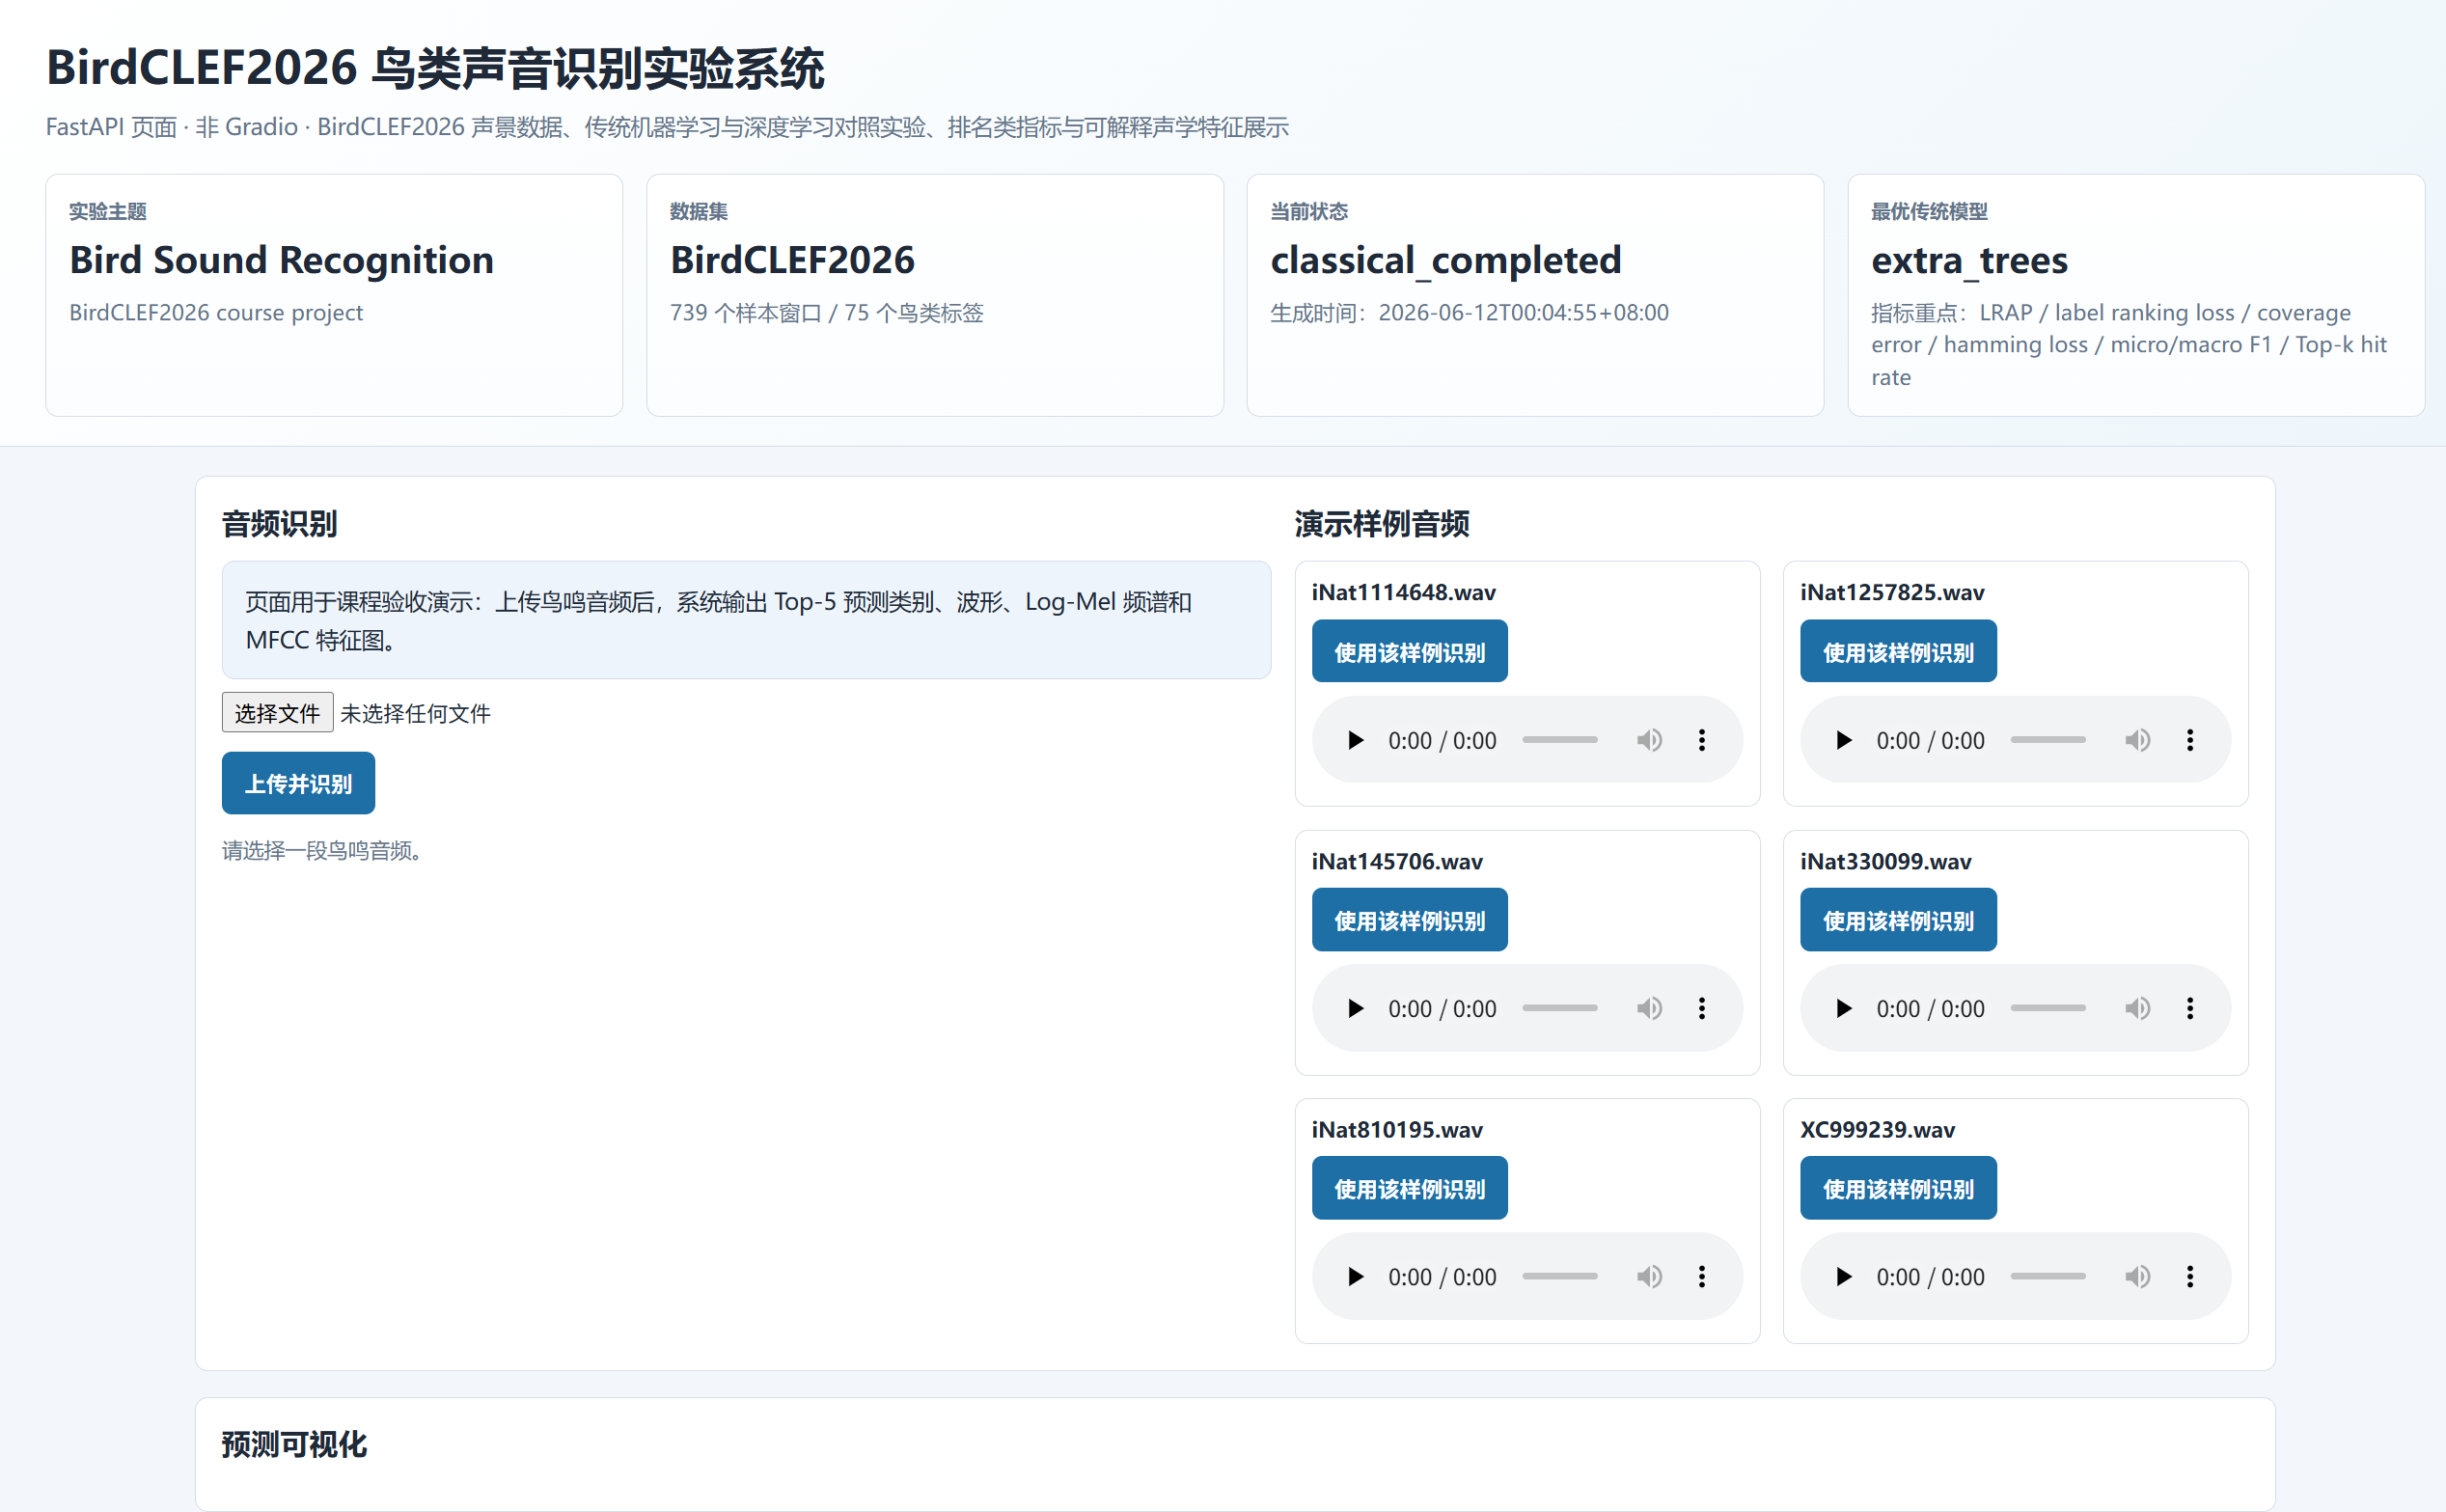
\includegraphics[width=\textwidth]{figures/lsw_dashboard_audio_module.png}
\caption{网页顶部概览与音频上传模块}
\label{fig:web-audio-module}
\end{figure}

\begin{figure}[H]
\centering
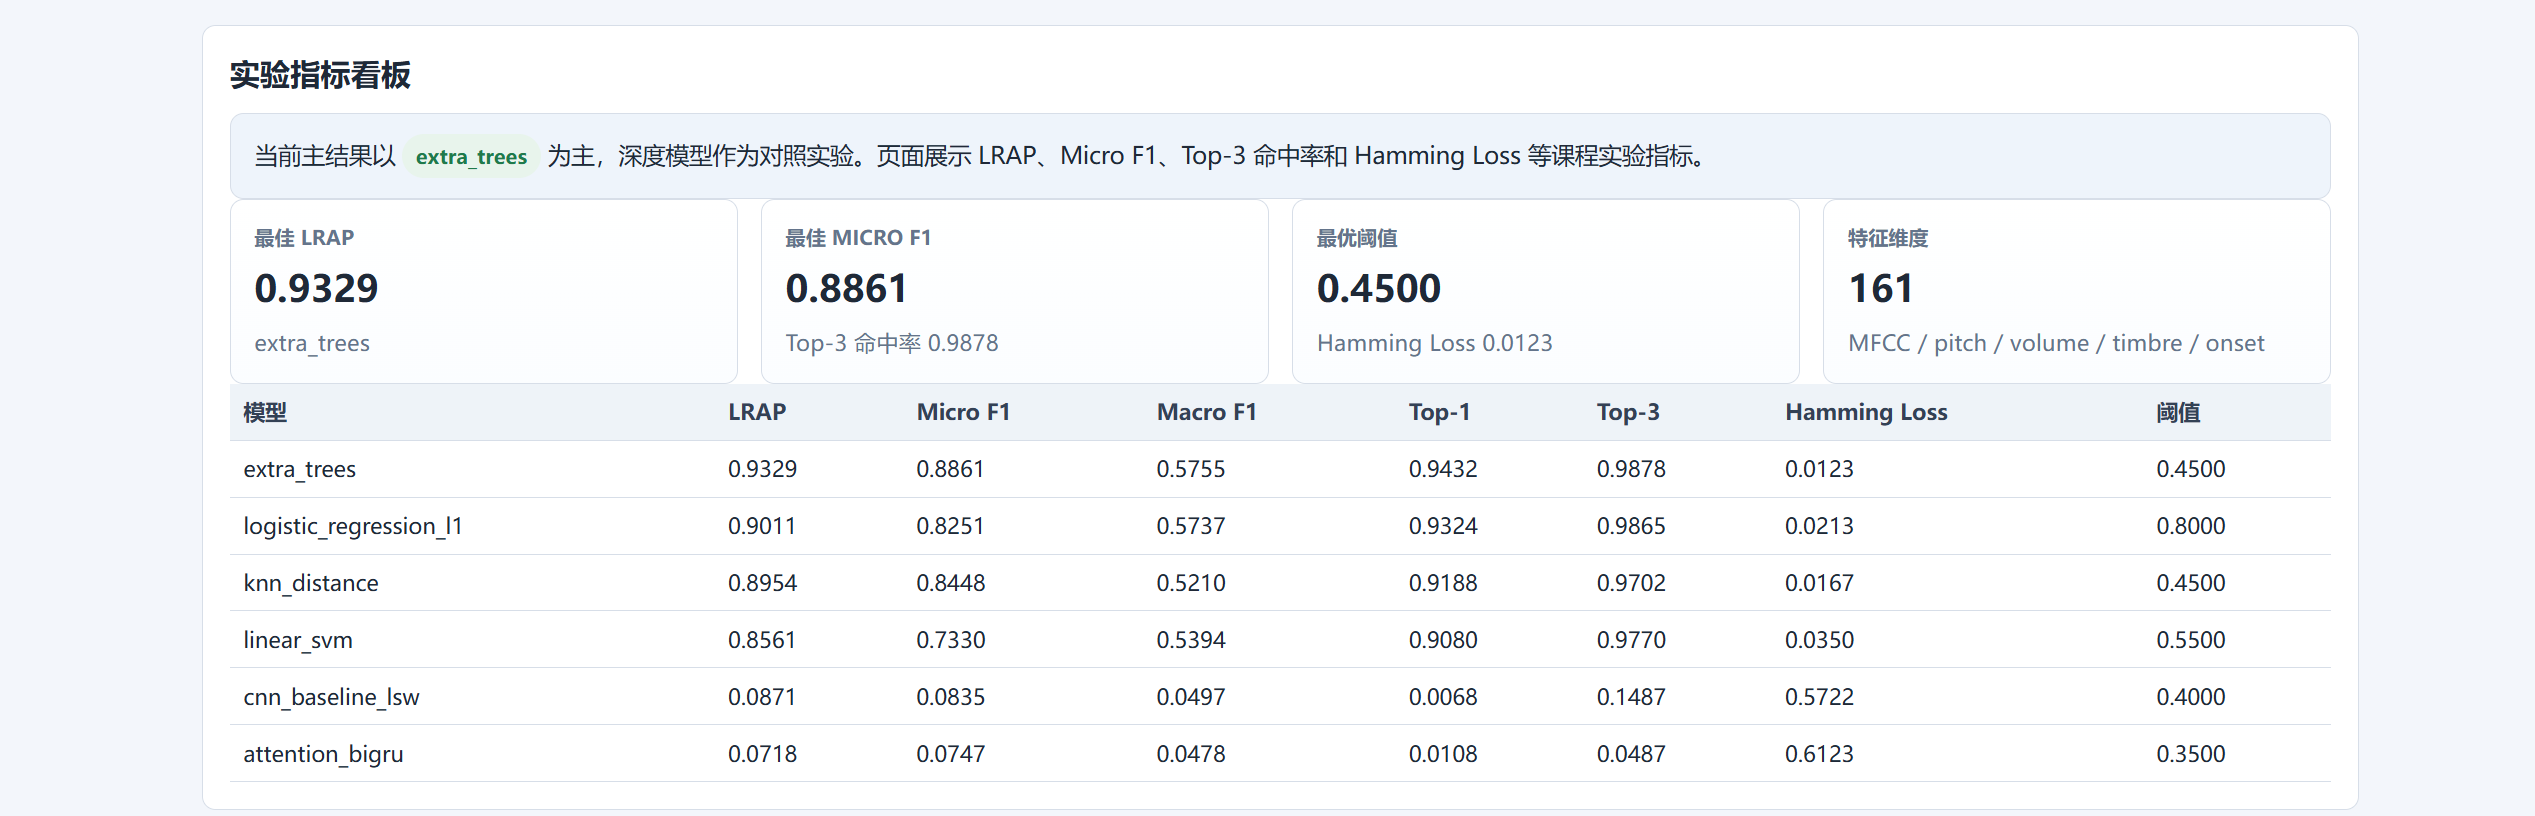
\includegraphics[width=\textwidth]{figures/lsw_dashboard_metrics_module.png}
\caption{模型指标看板模块}
\label{fig:web-metrics-module}
\end{figure}

\begin{figure}[H]
\centering
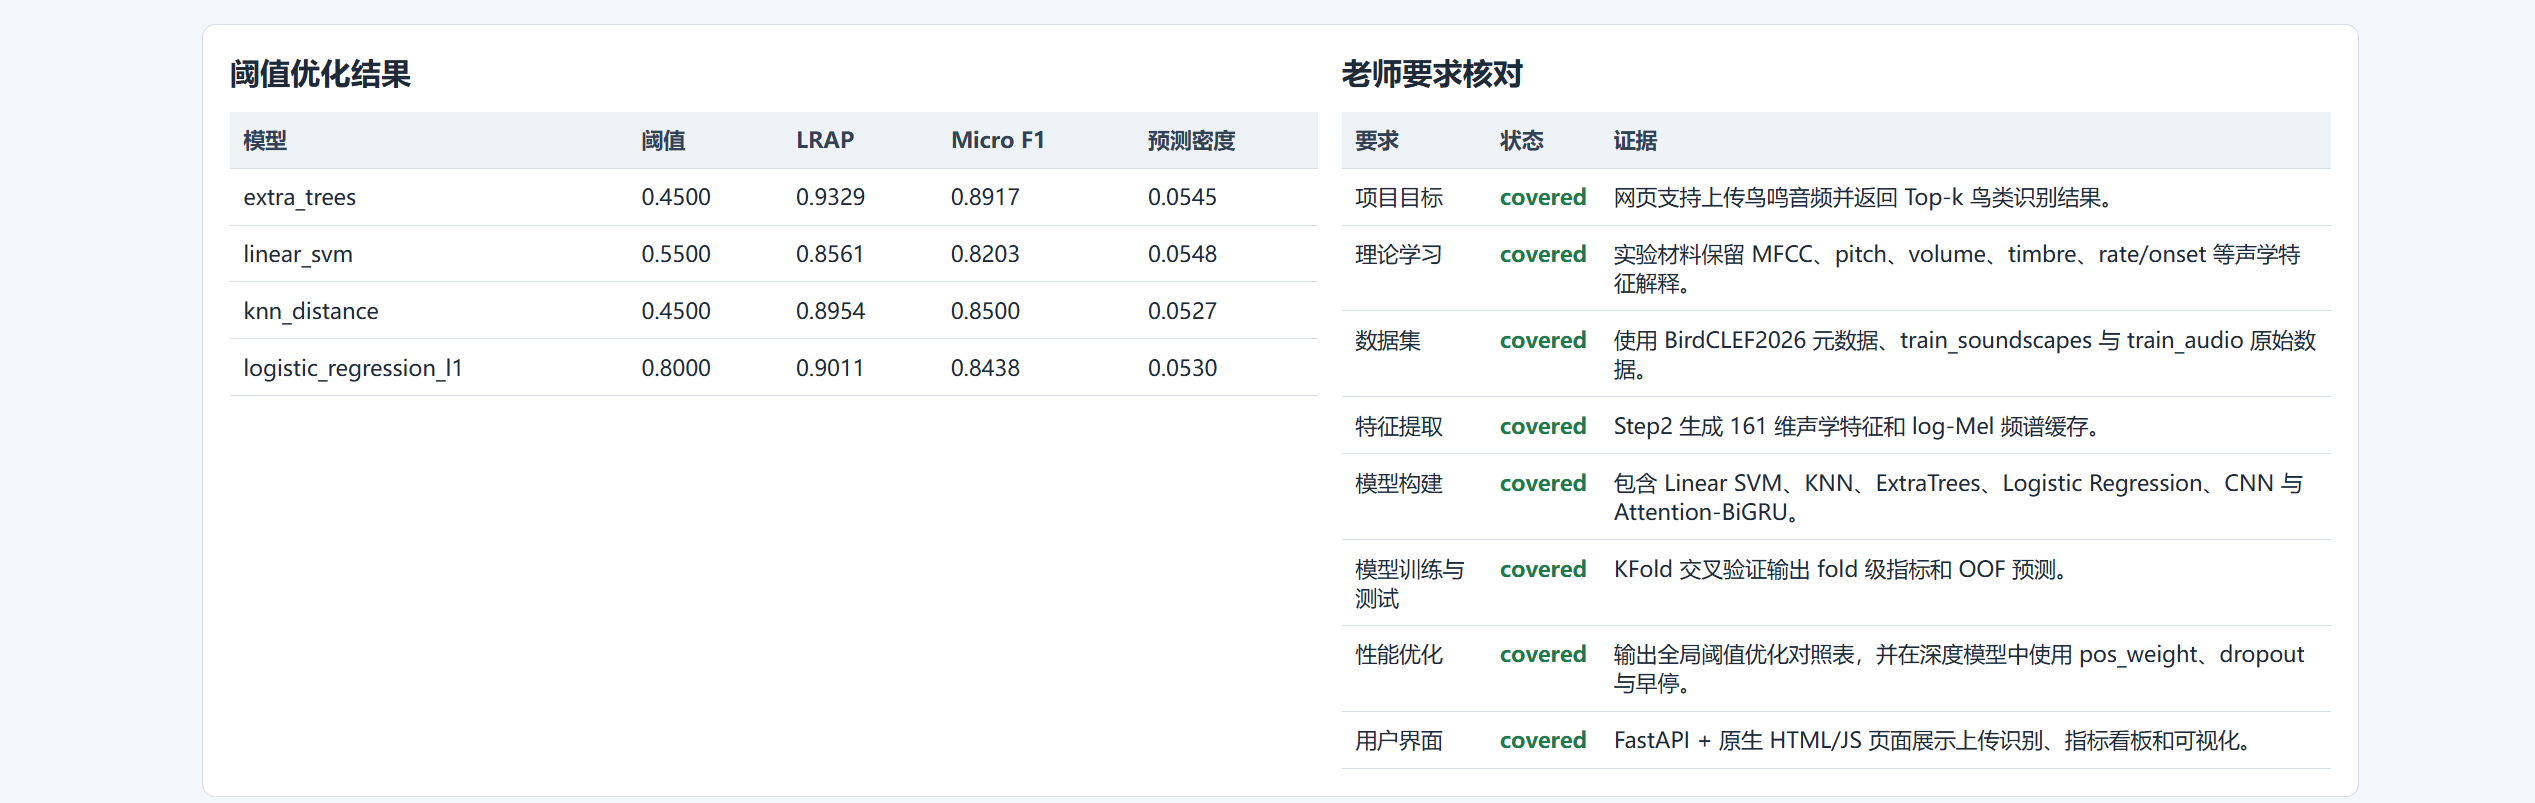
\includegraphics[width=\textwidth]{figures/lsw_dashboard_checklist_module.png}
\caption{阈值优化与课程要求核对模块}
\label{fig:web-checklist-module}
\end{figure}

\begin{figure}[H]
\centering
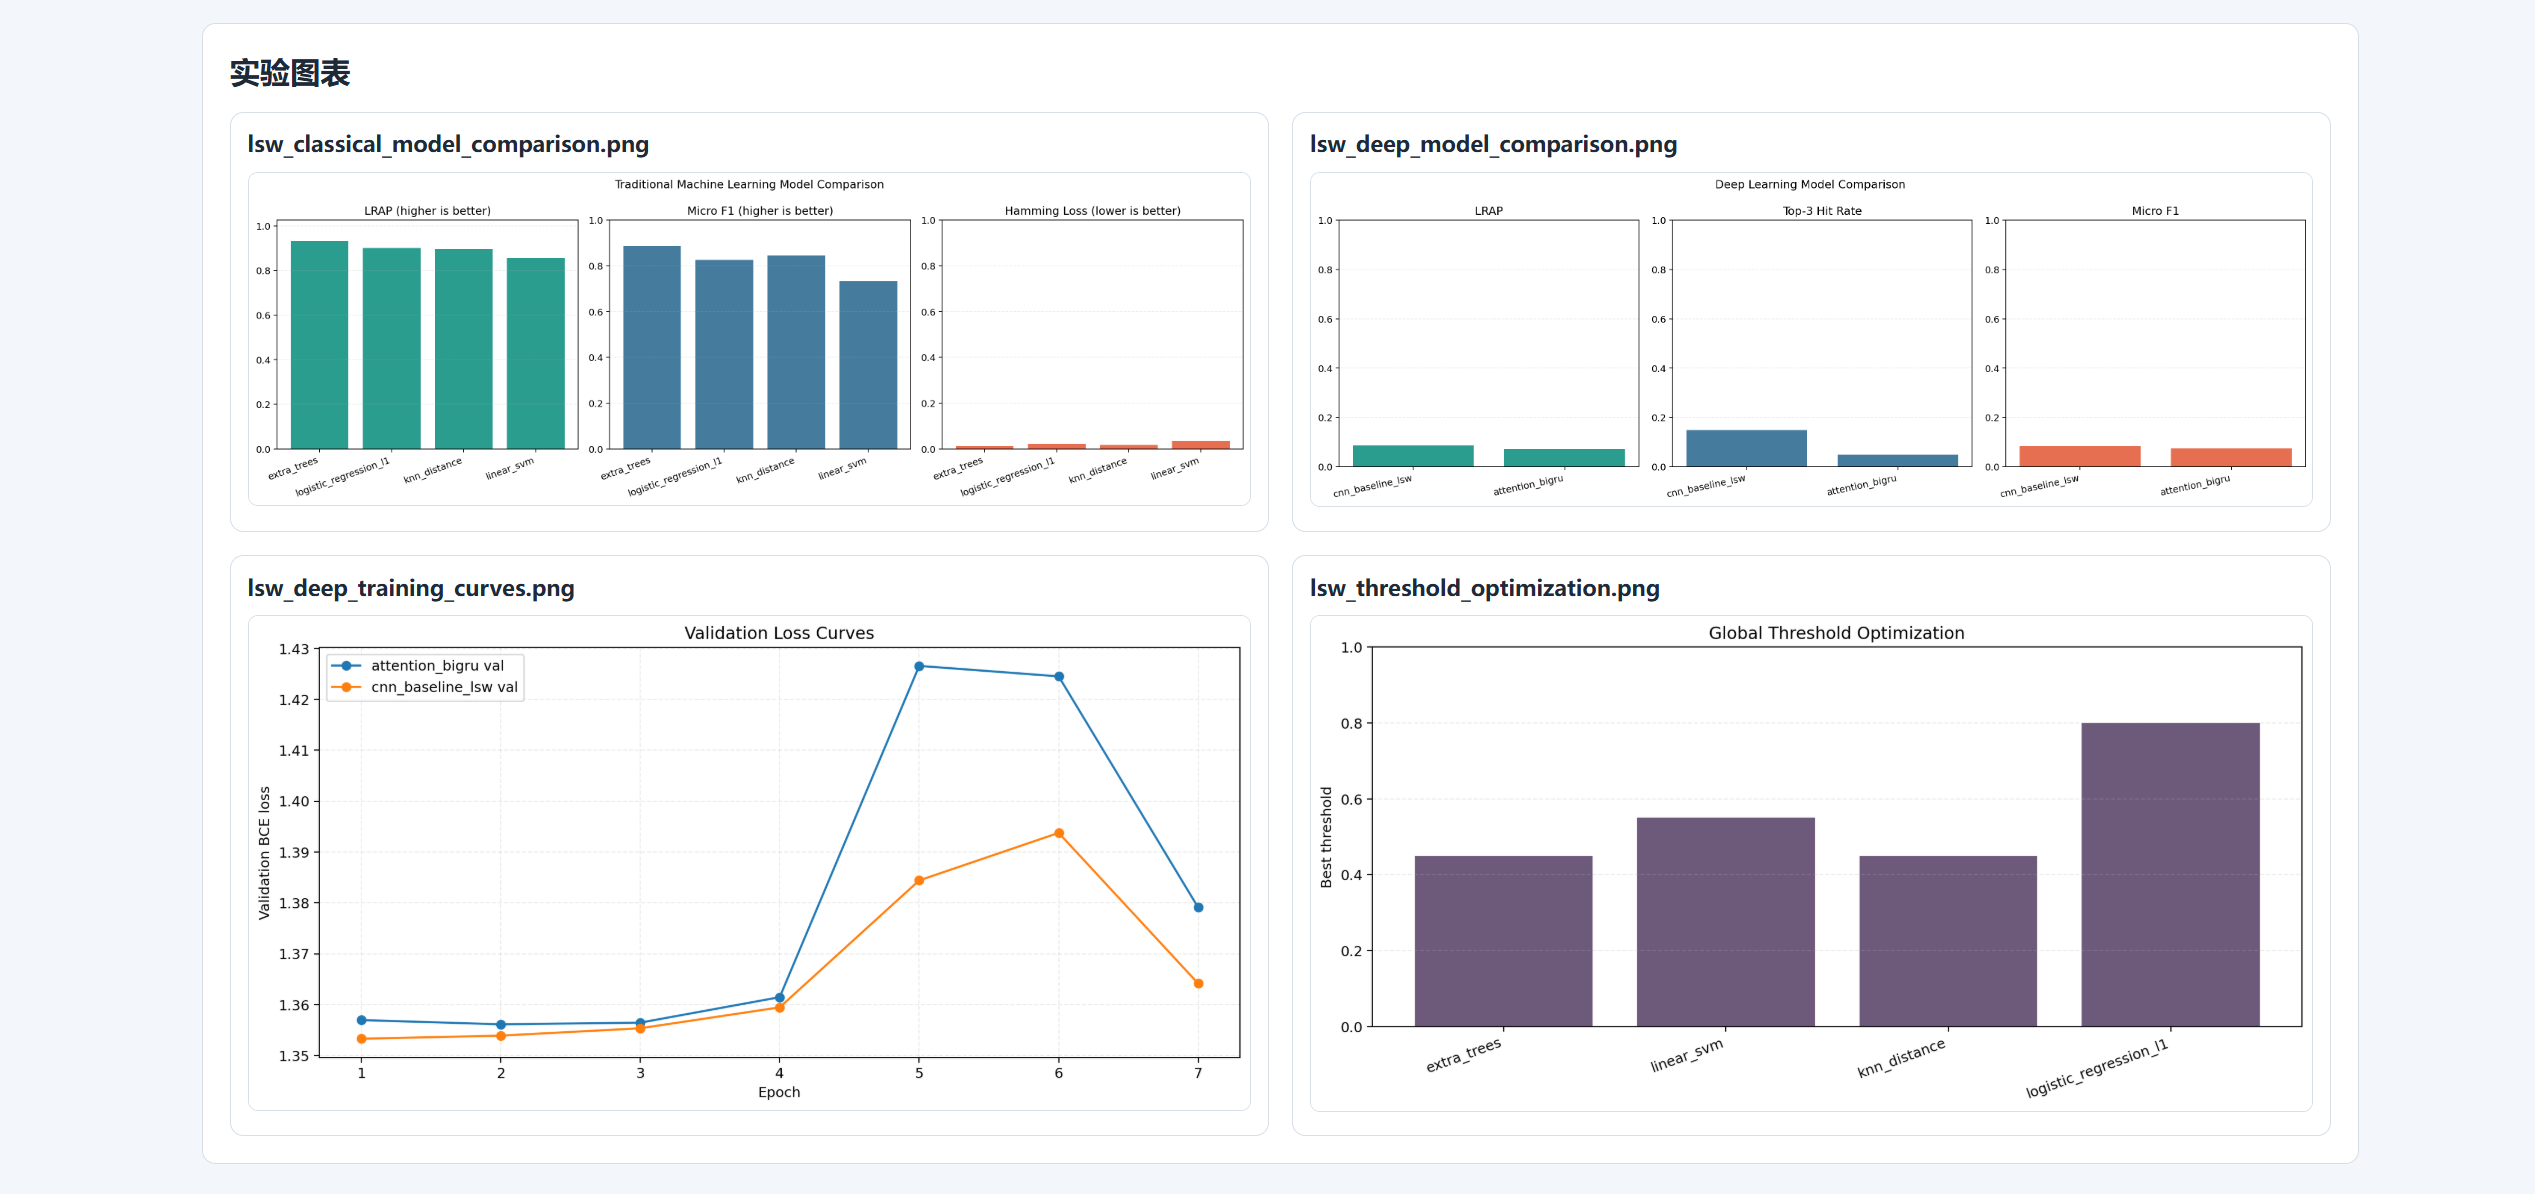
\includegraphics[width=\textwidth]{figures/lsw_dashboard_figures_module.png}
\caption{实验图表展示模块}
\label{fig:web-figures-module}
\end{figure}

网页的重点是把“声音识别过程”展示出来。用户上传音频后，系统会返回 Top-k 鸟类类别，同时生成波形、Log-Mel 频谱和 MFCC 图。波形对应原始时域信号，Log-Mel 频谱对应语音识别中常用的时频表示，MFCC 则对应传统声学特征。这样展示比只给一个类别名更清楚，也更符合本课程对声音特征提取的要求。

\subsection{网页演示流程说明}
课堂演示时，我们可以按“输入音频、观察特征、查看预测、解释指标”的顺序进行。先选择一个样例音频或上传一段新的鸟鸣文件，页面会把音频送到后端接口进行预处理。后端统一采样率和声道后，生成模型输入，并返回 Top-k 候选类别。这个过程对应真实声音识别系统中的前端处理、特征提取和分类决策。

预测结果之外，页面还会展示波形、Log-Mel 频谱和 MFCC。波形可以说明声音强弱和是否存在明显静音段；Log-Mel 频谱可以说明某些鸟鸣集中在高频还是低频，以及鸣叫是否呈现重复条纹；MFCC 图可以说明我们如何把复杂频谱进一步压缩为更适合传统模型使用的特征。对老师讲解时，可以先指出“我们不是只做了网页上传，而是把声音信号处理过程也可视化出来”，这样更能体现课程中的语音识别知识。

指标看板用于说明实验结果，而不是替代识别过程。看板中的 LRAP 和 Top-3 命中率解释候选列表质量，Hamming Loss 说明误报和漏报情况，阈值表说明我们做过性能优化。老师要求核对模块则把课程八项要求和对应证据放在一起，便于检查是否覆盖数据集、特征、模型、训练、优化和界面。

\subsection{部署与资源调度}
网页最终运行在远程服务器的 \texttt{127.0.0.1:7860}，并通过本地 SSH 隧道访问。为了避免与 GPU 训练冲突，我们让网页推理默认走 CPU，深度训练使用远程 4090D 显卡。这样网页推理速度会慢一些，但训练和演示可以同时保留。

\section{课程要求对应与完成情况}

结合实验代码、图表和网页演示，我们已经覆盖老师要求的八项内容。项目目标方面，网页可以上传鸟鸣音频并输出多标签 Top-k 识别结果；理论学习方面，报告解释了多标签建模、MFCC、pitch、volume、timbre、rate/onset 和排序指标；数据集方面，实验使用 BirdCLEF2026 相关数据和声景标签。特征提取部分实现了结构化声学特征和 log-Mel 频谱缓存；模型构建同时包含传统机器学习和深度学习；模型训练与测试统一使用 5 折交叉验证；性能优化包括全局阈值搜索、pos\_weight、dropout、早停和简单 SpecAugment；用户界面则由 FastAPI 页面完成演示。

从作业提交角度看，当前材料已经包含实验结果、图表、网页截图和报告正文，能够支撑课程验收。

我们在整理材料时尽量让每一项要求都有可检查证据。数据集部分有样本统计表和标签分布图，特征部分有特征家族表和网页可视化图，模型部分有六个模型的总表，训练测试部分有 5 折结果，优化部分有阈值对照表，界面部分有分模块网页截图。这样即使老师不运行代码，也可以通过报告看到完整实验链路；如果老师现场检查网页，也可以通过上传样例音频看到同一套流程。

\section{实验产物与复现说明}

\subsection{产物组织}
为了方便检查，我们把实验相关内容统一放在同一个目录下。表格类结果保存在 \texttt{artifacts/lsw/tables}，包括模型总表、传统模型交叉验证结果、深度模型 fold 结果、阈值优化表和实验 manifest。图像类结果保存在 \texttt{artifacts/lsw/figures}，包括模型对比图、训练曲线和阈值图。网页截图保存在 \texttt{artifacts/lsw/screenshots}，报告中引用的图片会同步复制到 \texttt{report/lsw\_report/figures}。

这种组织方式的好处是，报告、网页和实验结果不会混在一起。老师如果只看报告，可以直接查看 PDF；如果要检查原始实验输出，可以进入 artifacts 目录查看 CSV 和 PNG；如果要检查网页，则启动 FastAPI 服务后访问本地端口。我们在报告里引用的数值都来自这些产物文件，没有手工随意改动结果。

\subsection{复现实验流程}
复现实验时，先完成数据准备和特征提取，再运行传统模型和深度模型训练。传统模型主要依赖结构化特征表，训练速度较快；深度模型需要读取 log-Mel 频谱缓存，并在 GPU 上进行 5 折训练。训练完成后，脚本会生成汇总表、fold 级结果、阈值优化结果和图像。最后再运行报告资源脚本，把最新 CSV 和 PNG 转成 LaTeX 可引用的表格与图片。

网页复现则使用 FastAPI 启动。页面启动后会读取 artifacts 中的指标和图表，并提供样例音频识别接口。我们在截图前刷新了页面并强制重新加载图像资源，避免浏览器缓存旧图片导致中文标题显示异常。最终报告中的模块截图来自同一次刷新后的页面状态，和当前 artifacts 目录中的实验结果保持一致。

\section{结论与后续改进}

\subsection{主要结论}
本实验最直接的结论是：BirdCLEF2026 当前监督子集具有明显的小样本、多标签和类别不平衡特征，不能用单标签分类思维直接处理。我们在 5 秒窗口上建立多标签矩阵，并使用适合多标签任务的排序指标和阈值指标，能更真实地反映声景中多个鸟类同时出现的情况。

从模型结果看，结构化声学特征配合传统机器学习模型更适合这次任务。ExtraTrees 是综合最优模型，LRAP 为 0.9329，Micro F1 为 0.8862，Top-3 命中率为 0.9878。我们也完成了 CNN baseline 和 Attention-BiGRU 的 5 折 GPU 训练，但在当前样本规模下，深度模型表现弱于传统特征路线，所以报告中把它们作为对照实验，而不是主模型。

网页部分把实验结果、预测流程和声学可视化放在同一页面中。对老师演示时，可以先说明上传音频后的识别结果，再展示波形、Log-Mel 频谱和 MFCC 图，从语音识别/音频识别的角度解释模型为什么需要这些特征。

\subsection{局限性}
这套实验仍有几处局限。739 个监督窗口对 75 个标签而言偏少，深度模型很难稳定收敛。我们只尝试了两种轻量深度结构，没有做更系统的架构搜索。阈值优化目前采用全局阈值，还没有尝试 per-label threshold。网页推理为了和训练隔离，默认走 CPU，延迟不是最低。另一个需要改进的地方是，当前网页主预测模型使用深度检查点，更适合做演示接口；如果追求最佳识别效果，后续应把 ExtraTrees 等最佳传统模型包装成正式在线推理后端。

\subsection{后续改进方向}
后续如果继续完善，我们会优先从数据和声学特征两方面推进。一方面，可以增加更强的数据划分和标签清洗策略，减少噪声标签对模型的影响；另一方面，可以把网页里的可视化扩展为“波形 + Pitch + Onset + Timbre/Rate summary”的形式，让声音识别过程更直观。模型部分可以继续尝试 per-label threshold 和输出校准，也可以把最佳传统模型接入网页正式推理接口。深度网络不是本报告的重点，但后续可以考虑使用预训练音频 backbone，再比较它和结构化声学特征路线的差异。

总体来看，我们完成了一个面向课程要求的鸟类声音识别实验系统。实验结果比较清楚：在当前 BirdCLEF2026 小样本多标签条件下，结构化声学特征与传统机器学习的组合更可靠，也更容易解释。深度模型虽然没有取得更高分数，但它提供了频谱端到端路线的对照结果，使整个实验结论更完整。

\end{document}
